\documentclass[lettersize,journal]{IEEEtran}
\usepackage[caption=false,font=normalsize,labelfont=sf,textfont=sf]{subfig}
\usepackage{stfloats}
\usepackage{verbatim}
\hyphenation{op-tical net-works semi-conduc-tor IEEE-Xplore}
\def\BibTeX{{\rm B\kern-.05em{\sc i\kern-.025em b}\kern-.08em
    T\kern-.1667em\lower.7ex\hbox{E}\kern-.125emX}}
\usepackage{balance}

\usepackage[backend=biber,style=numeric]{biblatex} % or 'authoryear' or another style
\addbibresource{bibliography.bib}

\usepackage{graphicx}
\usepackage{amsmath,amssymb,amsfonts}
\usepackage{amsthm}
\usepackage{algorithmic}
\usepackage{textcomp}
\usepackage{float}
\usepackage{etoolbox}
\usepackage{hyperref}
\usepackage{orcidlink}
\usepackage{tikz}
\usepackage{fontawesome}
\usepackage{subcaption}
\usepackage{url}
\usepackage{listings}
\usepackage{pdfpages}
\usepackage[english]{babel}
\usepackage{scalerel}
\usepackage{xcolor,colortbl}
% \usepackage{cite}
\usepackage[linesnumbered,ruled,vlined]{algorithm2e}
\usepackage{amsmath}
\usepackage{amssymb}
\usepackage{multirow}
\usepackage{array}



\newtheorem{lemma}{Lemma}
\newtheorem{corollary}{Corollary}
\theoremstyle{definition}
\newtheorem{definition}{Definition}
\newtheorem{theorem}{Theorem}

\begin{document}

\title{Federated Distributed Key Generation}
% \author{Anonymous Authors}

% \author{Stanislaw Baranski, Julian Szymanski
% \thanks{Stanislaw Baranski and Julian Szymanski are with Department of Electronic, Telecommunication and Informatics, Gdansk University of Technology, Gdansk, 
% Poland}
% }

\author{Stanislaw Baranski\,\orcidlink{0000-0001-7181-8860}     
    \and
    Julian Szymanski\,\orcidlink{0000-0001-5029-6768}
    \thanks{Stanislaw Baranski and Julian Szymanski are with Department of Electronic, Telecommunication and Informatics, Gdansk University of Technology, Gdansk, 
Poland}
}
    

\date{}
\maketitle
\begin{abstract}
    Distributed Key Generation (DKG) is vital to threshold-based cryptographic protocols such as threshold signatures, secure multiparty computation, and i-voting. Yet, standard \((n,t)\)-DKG requires a known set of \(n\) participants and a fixed threshold \(t\), making it impractical for public or decentralized settings where membership and availability can change.

    We introduce Federated Distributed Key Generation (FDKG), which relaxes these constraints by allowing each participant to select its own “guardian” set, with a local threshold to reconstruct that participant’s partial key. FDKG generalizes DKG and draws inspiration from Federated Byzantine Agreement, enabling dynamic trust delegation with minimal message complexity (two rounds). The protocol's liveness can tolerate adversary that controls up to $k - t + 1$ nodes in every guardian set. The paper presents a detailed protocol, a formal description of liveness, privacy, and integrity properties, and a simulation-based evaluation showcasing the efficacy of FDKG in mitigating node unreliability.

    In a setting of 100 parties, a 50\% participation rate, 80\% retention, and 40 guardians, the distribution phase incurred a total message size of 332.7 kB ($\mathcal{O}(n\,k)$), and reconstruction phase 416.56 kB ($\mathcal{O}(n\,k)$. Groth16 client-side proving took about 5 s in the distribution phase and ranged from 0.619 s up to 29.619 s in the reconstruction phase. 
    
    Our work advances distributed cryptography by enabling flexible trust models for dynamic networks, with applications ranging from ad-hoc collaboration to blockchain governance.
\end{abstract}

\section{Introduction}

Distributed cryptographic systems often depend on Distributed Key Generation (DKG) to achieve decentralization without single points of trust. Most i-voting systems rely on DKG to distribute the encryption keys that secure election privacy~\cite{baranskiTrustCentricApproachQuantifying2024}. However, traditional DKG approaches are not well-suited to dynamic environments with unreliable or partially available nodes. This limits their application in dynamic, decentralized systems where trust relationships often evolve and are not uniform or predefined. 
In a standard $(n, t)$-DKG protocol, a set of $n$ nodes collectively generates a secret whose shares are spread over the nodes, allowing any subset larger than $t$ to reconstruct the secret, while smaller subsets do not have any knowledge about it.
Standard DKG schemes assume a predefined number of participants $n$ and a threshold $t$. 
When participation is voluntary (e.g., in public protocols), the actual number of participants remains unknown until the end of the key distribution phase. If fewer users join than expected, the preselected threshold may not be achievable, making the system unusable.

To overcome these limitations, we introduce \emph{Federated Distributed Key Generation (FDKG)}, a novel protocol that extends DKG to scenarios where the actual number of participants remains unknown until the end of the key distribution phase and nodes are  unequally trusted. 

FDKG employs \emph{Guardian Sets}, allowing participants to delegate key-reconstruction responsibilities to a trusted subset of nodes. Formally, an $(n, p, t, k)$-FDKG protocol involves $n$ nodes, of which a fraction $p$ participate in generating partial secret keys. Each node’s key share is distributed among a guardian set of size $k$, using a $t$-out-of-$k$ secret sharing scheme. During reconstruction, only a sufficient fraction of those who participated need to supply their partial keys or shares. Subsets below that threshold gain no information about the final key.

FDKG generalizes the traditional $(n, t)$-DKG protocol. The standard DKG is a special case $(n, 1, t, n-1)$, where all nodes participate and every node’s guardian set is the entire rest of the network.

This novel approach provides:
\begin{itemize}
    \item \textbf{Dynamic Participation}: FDKG allows a set of participants to join the key generation process and establish keys with a single round of message exchange, without prior knowledge of all members.
    
    \item \textbf{Flexible Trust Model}: Each participant can choose its own ``Guardian Set'' of trusted nodes, making the protocol more amenable to decentralized settings with diverse or evolving trust relationships.

    \item \textbf{Resilience to Node Unavailability}: FDKG uses threshold cryptography to ensure that as long as enough guardians remain honest, the global key can be reconstructed—even if some participants go offline or behave maliciously.
\end{itemize}

Figure~\ref{fig:trust-models} illustrates the differences between centralized trust, distributed trust, and the federated trust model introduced in this paper. Unlike centralized and distributed models, the federated model enables participants to delegate trust to subsets of nodes, aligning with the dynamic and decentralized requirements of modern systems.

\begin{figure}
    \centering
    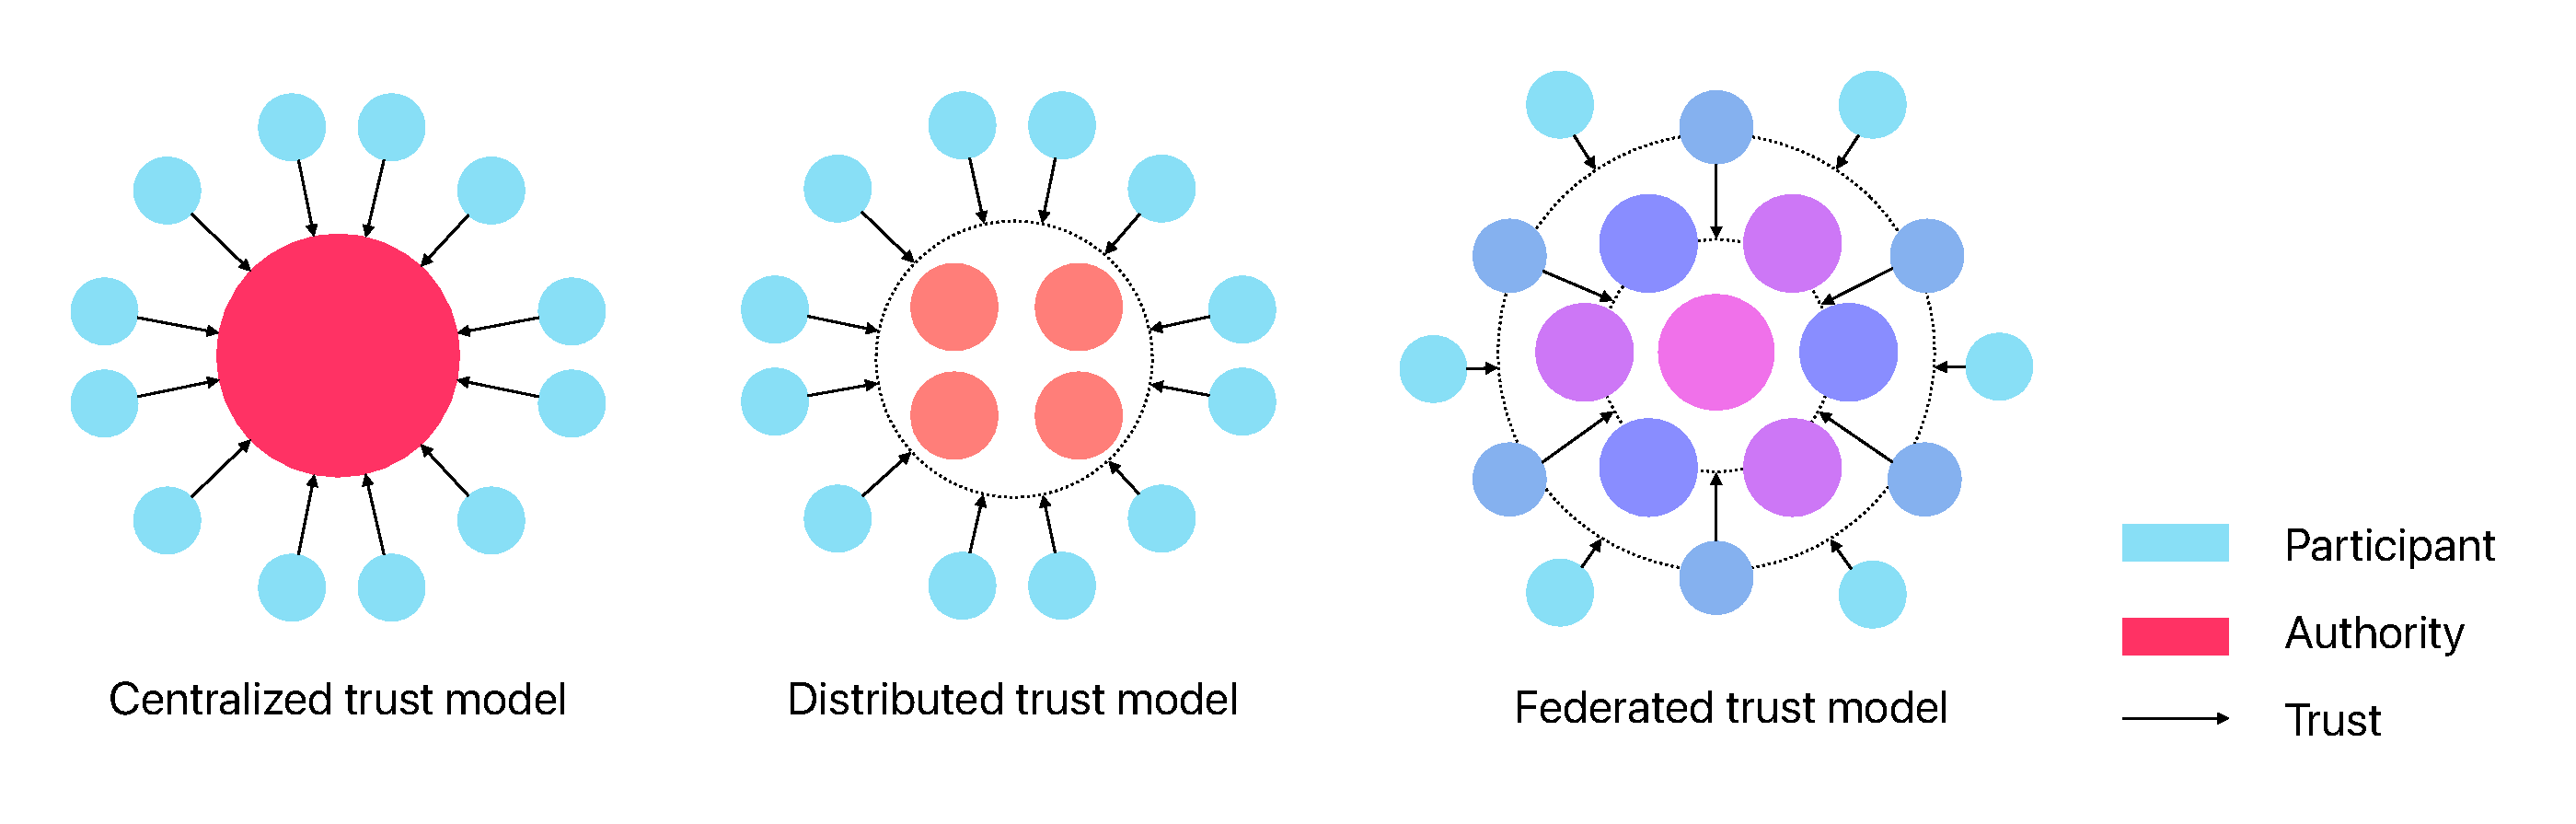
\includegraphics[width=0.5\textwidth]{federated_trust_model.pdf}
    \caption{Comparison of trust models in distributed systems: centralized trust (one authority), distributed trust (multiple authorities), and federated trust (peer-to-peer with individually chosen trusted groups).}
    \label{fig:trust-models}
\end{figure}

In this paper, we detail the FDKG protocol, discuss its security properties, and demonstrate its practical application through a peer-to-peer internet voting scheme. We show how leveraging trust relationships at the participant level can yield robust key generation without sacrificing privacy. Our main contribution is the introduction of Federated Distributed Key Generation (FDKG) as a generalization of standard DKG with individually chosen guardian sets.

This paper makes the following contributions:
\begin{itemize}

    \item Formalizing FDKG, including its liveness, privacy, and integrity properties.
    \item Demonstrating the protocol’s performance and robustness via extensive simulations under diverse network topologies, participation rates, and retention conditions.
    \item Integrating FDKG into an end-to-end internet voting scheme featuring threshold ElGamal encryption, zkSNARK-based verifiability, and a fully open-source implementation.
\end{itemize}

The remainder of this paper is organized as follows.  
Section~\ref{sec:related_work} reviews the related work on DKG and decentralized key generation.  
Section~\ref{sec:preliminaries} presents key cryptographic tools used in our protocol.  
Section~\ref{sec:fdkg} describes the FDKG protocol in detail.  
Section~\ref{sec:security_properties} defines our security properties and shows how FDKG meets them.  
Section~\ref{sec:liveness_simulations} discusses extensive simulation results. 
Section~\ref{sec:voting_scheme} applies FDKG to a voting scenario.
Section~\ref{sec:performance_evaluation} assesses the performance of the key components.
Section~\ref{sec:deployments} outlines possible deployment strategies.
Finally, Sections~\ref{sec:limitations-and-future} and~\ref{sec:discussion-conclusion} offers concluding remarks and open directions.


\section{Related Work}\label{sec:related_work}

Distributed Key Generation (DKG) has been extensively studied in cryptography. Early work focused on secure and robust schemes for generating shared secret keys based on discrete logarithm-based cryptosystems~\cite{gennaroSecureDistributedKey1999}. These schemes typically employ Shamir's Secret Sharing (SSS)~\cite{shamirHowShareSecret1979} to distribute key shares among participants, which are subsequently combined to recover the shared secret.

While considerable research has addressed enhancing DKG for reliable operation in adversarial environments like the Internet~\cite{kateDistributedKeyGeneration2012,dasPracticalAsynchronousDistributed2022,dasPracticalAsynchronousHighthreshold2022,zhangPracticalAsynchronousDistributed2023}, this work focuses on a different problem: enabling users to interactively establish a distributed key pair within a maximum of two rounds, without prior knowledge of the other participants.  The challenge arises from Shamir secret sharing, which requires a known polynomial degree for secret sharing.  If the number of participants remains unknown until the end of a round, this degree cannot be predetermined.

Dynamic DKG schemes~\cite{delerableeDynamicThresholdPublickey2008} were designed to address this issue, allowing parties to join and leave the protocol at any time. However, these schemes often necessitate multiple rounds of interaction, which can be impractical when human input is required.

This paper introduces Federated Distributed Key Generation (FDKG), a protocol that innovates by using dynamic, participant-defined "guardian sets." This approach enables key reconstruction even in unpredictable or unreliable network settings.  This flexibility generalizes traditional DKG protocols, enhancing adaptability while preserving security and resilience.

Our approach draws inspiration from Federated Byzantine Agreement (FBA) protocols, which underpin the Stellar Consensus Protocol~\cite{mazieresStellarConsensusProtocol2015}, a core component of a prominent blockchain network. FBA enables open and dynamic participation by allowing nodes to independently select their trusted peers, forming "quorum slices." This flexible trust model allows nodes to make trust decisions based on individual preferences.  As a node is included in more quorum slices (or guardian sets), its perceived trustworthiness within the network increases, reinforcing its role and enhancing overall network reliability.

Most internet voting protocols mitigate single points of failure by distributing decryption keys among multiple authorities, often termed Key Holders~\cite{barandiaranDecidimTechnopoliticalNetwork2024,adidaHeliosWebbasedOpenAudit2008,haenniCHVoteProtocolSpecification2017,larraiaSVoteControlComponents2022} or Trustees~\cite{cortierBeleniosSimplePrivate2019,mattbeckerProofVoteEndtoend2018}.  Election privacy is maintained as long as a threshold of these authorities remains non-collusive. However, these approaches rely on a predefined set of trusted authorities, making them vulnerable to attacks, collusion, or absence during key reconstruction, potentially halting the entire voting process.

The primary motivation for developing FDKG is to create a more robust and decentralized foundation for internet voting protocols, analogous to how FBA has enhanced decentralization in the Ripple blockchain~\cite{mazieresStellarConsensusProtocol2015}. FDKG decentralizes trust by shifting it to the voter level, empowering each participant to select their own trusted parties (guardian sets) for key reconstruction. This eliminates reliance on a single authority or fixed set of trustees, significantly improving system flexibility and resilience to node unavailability.

% Party
\newcommand{\PartySecretKey}[1]{\ensuremath{s_{#1}}}
\newcommand{\Party}[1]{\ensuremath{P_{#1}}}
\newcommand{\Parties}{\ensuremath{\mathbb{P}}}
\newcommand{\VotesSize}{\ensuremath{|\mathbb{V}}|}

% Voting keys
\newcommand{\PublicKey}{\textbf{E}}
\newcommand{\SecretKey}{\textbf{d}}

% Partial voting keys
\newcommand{\PartialSecretKey}[1]{\ensuremath{d_{#1}}}
\newcommand{\PartialPublicKey}[1]{\ensuremath{E_{#1}}}


\newcommand{\SharePartialSecretKey}[2]{\ensuremath{[d_{#1}]_{#2}}}

% Ciphertexts
\newcommand{\EncryptedSharePartialSecretKey}[2]{\ensuremath{C_{#1,#2}}}
\newcommand{\SetOfEncryptedPartialSecretKeys}{\ensuremath{\mathbb{C}}}
\newcommand{\SetOfFDKG}{\ensuremath{\mathbb{D}}}
\newcommand{\SetOfSharesOfPartialDecryption}{\ensuremath{\mathbb{C}}}
\newcommand{\Voters}{\ensuremath{\mathbb{V}}}
\newcommand{\Tallies}{\ensuremath{\mathbb{T}}}
% Shares
\newcommand{\IthSecretKey}[1]{\ensuremath{d_{#1}}}
\newcommand{\IthPublicKey}[1]{E_{#1}}

% Private channel
\newcommand{\DecryptionUsingOf}[2]{\ensuremath{\texttt{Dec}_{#1}(#2)}}
\newcommand{\EncryptionUsingOf}[2]{\ensuremath{\texttt{Enc}_{#1}(#2)}}

\newcommand{\ProofPS}[1]{\ensuremath{\textrm{PROOF}_{\PartialSecretKey{#1}}}}

\newcommand{\ProofSPS}[2]{\ensuremath{\textrm{PROOF}_{\SharePartialSecretKey{#1}{#2}}}}

\newcommand{\ProofFDKG}[1]{\ensuremath{\textrm{PROOF}_{\textrm{FDKG}_{#1}}}}

\newcommand{\ProofFDKGInformal}{"Given \PartialPublicKey{i}, \EncryptedSharePartialSecretKey{i}{j} and $\Party{j} \in \GuardianSetOf{i}$, I know $f_i = a_0, \dots, a_{t-1}$, $r1_1,\dots,r1_k$, and $r2_1,\dots,r2_k$, s.t. $\PartialPublicKey{i}=a_0G$ and the \EncryptedSharePartialSecretKey{i}{j} is an encrypted value of a polynomial $f_i$ applied to $j$"}

\newcommand{\ProofBALLOT}[1]{\ensuremath{\textrm{PROOF}_{\textrm{\Ballot{#1}}}}}

\newcommand{\ProofBALLOTInformal}{"Given \PublicKey{} and \Ballot{i} = $(C1, C2)$, I know \BlindingFactor{i}, and \Vote{i} s.t. $\Vote{i} \in \{2^0, 2^j, \ldots, 2^{(l-1)j}\}$ and $\Ballot{i} = (\BlindingFactor{i} G,\ \BlindingFactor{i} \PublicKey{} + \Vote{i})$"}

\newcommand{\ProofPD}[1]{\ensuremath{\textrm{PROOF}_{\PartialDecryptionFrom{#1}}}}

\newcommand{\ProofPDInformal}{"Given $\TotalA{}, \PartialDecryptionFrom{i}, \PartialPublicKey{i}$, I know a partial decryption key $\PartialSecretKey{i}$ s.t. $\PartialPublicKey{i} = \PartialSecretKey{i} G$ and $\PartialDecryptionFrom{i} = \PartialSecretKey{i} \TotalA{}$"}

\newcommand{\ProofPDS}[2]{\ensuremath{\textrm{PROOF}_{\SharePartialDecryptionFromTo{#1}{#2}}}}

\newcommand{\ProofPDSInformal}{"Given $\SharePartialDecryptionFromTo{j}{i}, \EncryptedSharePartialSecretKey{j}{i}, \TotalA$, I know a secret key $\PartySecretKey{i}$ s.t. $\SharePartialDecryptionFromTo{j}{i} = \TotalA  \SharePartialSecretKey{j}{i}$ where $\SharePartialSecretKey{j}{i} = \DecryptionUsingOf{\PartySecretKey{i}}{\EncryptedSharePartialSecretKey{j}{i}}$"}


\newcommand{\Ballot}[1]{\ensuremath{B_{#1}}}

\newcommand{\Generator}[1]{\ensuremath{H_{#1}}}
\newcommand{\BlindingFactor}[1]{\ensuremath{r_{i}}}
\newcommand{\Vote}[1]{\ensuremath{v_{#1}}}

\newcommand{\GuardianSetOf}[1]{\ensuremath{\mathbb{G}_{#1}}}
\newcommand{\TotalA}{\ensuremath{C1}}
\newcommand{\TotalB}{\ensuremath{C2}}
\newcommand{\BallotA}[1]{\ensuremath{C1_{#1}}}
\newcommand{\BallotB}[1]{\ensuremath{C2_{#1}}}

\newcommand{\G}{\ensuremath{G}}


% Partial Decryption Results
\newcommand{\SharePartialDecryptionFromTo}[2]{\ensuremath{[\mathrm{PD}_{#1}]_{#2}}}

\newcommand{\PartialDecryptionFrom}[1]{\ensuremath{\mathrm{PD}_{#1}}}


\section{Preliminaries}\label{sec:preliminaries}

This section outlines the core cryptographic concepts and tools that serve as building blocks of our FDKG protocol.


% Table of Notations
\begin{table}[!t]

\caption{Summary of Notations}
\label{tab:notations}
\begin{tabular}{>{\centering\arraybackslash}p{.2\linewidth}p{.7\linewidth}}
\hline
\textbf{Notation} & \multicolumn{1}{c}{\textbf{Description}} \\
\hline

\Parties          & Set of all parties $\Party{i} \in \Parties$ in the system \\


\Party{i},\PartySecretKey{i} & Public and secret keys used to authenticate $i$-th party, where $\Party{i}=\PartySecretKey{i} \G$  \\

\hline
$\SetOfFDKG \subseteq \Parties$ & Subset of parties involved in the 1. FDKG phase  \\

\PartialPublicKey{i},\PartialSecretKey{i}      & Partial encryption (public) and decryption (secret) keys of \Party{i}. $\PartialPublicKey{i}=\PartialSecretKey{i} \G$, where $\PartialSecretKey{i}$ is a random ephemeral (per vote) scalar value.  \\

\PublicKey{}, \SecretKey{}    & Voting public (encryption) and secret (decryption) keys, that is a sum of partial encryption keys \PartialPublicKey{i}, and decryption keys \PartialSecretKey{i} accordingly \\

$\GuardianSetOf{i}$ & Guardian set is a subset of parties  selected by \Party{i} that can recreate \Party{i}'s part of the decryption key \PartialSecretKey{i}.  $\GuardianSetOf{i} \subseteq \Parties \setminus \Party{i}$ \\

$k = |\GuardianSetOf{}|$                 & Total number of parties in a guardian set \\

$t$                 & Threshold number to reconstruct the shared secret \\

\SharePartialSecretKey{i}{j}      & Share of partial decryption (secret) key, from \Party{i} to \Party{j}   \\

\EncryptedSharePartialSecretKey{i}{j} & Encrypted partial decryption key share, from \Party{i} to \Party{j}  \\

\hline
$\Tallies \subseteq \Parties$ & Subset of parties  participating in the 3. Online Tally phase \\

\hline
$\texttt{Enc}_{\Party{i}}, \texttt{Dec}_{\PartySecretKey{i}}$ & Public key encryption for \Party{i} and decryption using the corresponding secret key $\PartySecretKey{i}$, as described in Section~\ref{private-channel} \\

$\Delta$ & A helper value used to encode a scalar value to a point on a curve \\

\EncryptedSharePartialSecretKey{i}{j} & Encrypted partial decryption key share, from \Party{i} to \Party{j}  \\

\hline
\ProofFDKG{i} & zkSNARK proof of correctness of (\PartialSecretKey{i}, \EncryptedSharePartialSecretKey{i}{}) \\

\ProofPS{i} & zkSNARK of partial secret \PartialSecretKey{i} \\

\ProofSPS{i}{j} & zkSNARK of share of partial secret \SharePartialSecretKey{i}{j} \\

\hline

\end{tabular}
\end{table}

\subsection*{Secret Sharing}
Secret sharing is a fundamental technique used in DKG to distribute a secret key $s$ among $n$ participants. Shamir's Secret Sharing (SSS) enables a dealer to distribute a secret key $s$ by sampling a random polynomial $\mathbf{f}(X) = a_0 + a_1X + a_2X^2 + \dots + a_{t-1}X^{t-1}$, where $a_0, a_1, \dots, a_{t-1}$ are random elements of a field $\mathbb{F}_q$. Here, the secret key is $s=a_0=\mathbf{f}(0)$, and $t-1$ denotes the degree of the polynomial. To share the secret key, the dealer computes shares by evaluating $\mathbf{f}(i)$ for each participant $i \neq 0$. The secret $s$ can be recovered by any $t$ or more participants by using Lagrange interpolation.

\subsection*{Distributed Key Generation}
To avoid centralising the role of the dealer (and revealing the secret value $s$), the generation of polynomial $\mathbf{f}(X) \in_R \mathbb{Z}_q[X]$ is distributed among all parties $\mathbb{P}$. Each party selects a random polynomial $f_{i}(X) \in \mathbb{Z}_q[X]$, and the final polynomial is the sum of these individual polynomials: 
\begin{equation}
  \mathbf{f}(X)=\sum_{i=1}^{n}f_i(X)  
\end{equation}
Consequently, the secret (decryption) key $\mathbf{d}$ and public (encryption) key $\mathbf{E}$ are defined as: 
\begin{equation}
\mathbf{d}=\mathbf{f}(0)\ \textrm{and}\ \mathbf{E}=\mathbf{d} \G
\end{equation}
 
To prevent arbitrary submissions by parties, Publicly Verifiable Secret Sharing (PVSS) is used, incorporating zero-knowledge proofs to validate the correctness of shared values \cite{goosSimplePubliclyVerifiable1999}.


\subsection{zk-SNARKs}

Zero-Knowledge Succinct Non-Interactive Arguments of Knowledge (zk-SNARKs) enable a prover to demonstrate the validity of a statement to a verifier without revealing any information beyond the validity of the statement itself~\cite{grothSizePairingBasedNoninteractive2016}. A zk-SNARK for an arithmetic circuit $C$, characterized by a relation $\mathcal{R}_C$ and a language $\mathcal{L}_C$, is defined as follows:
\begin{itemize}
    \item $\textrm{(pk,vk)} \gets \textrm{Setup}(1^\lambda,C)$: Given a security parameter $\lambda$ and the circuit $C$, this algorithm generates a proving key $\textrm{pk}$ and a verification key $\textrm{vk}$.
    \item $\pi \gets \textrm{Prove}(\textrm{pk}, \vec{s}, \vec{w})$: Given the proving key $\textrm{pk}$, a statement $\vec{s}$ and a witness $\vec{w}$ (where $(\vec{s},\vec{w}) \in \mathcal{R}_C$), this algorithm produces a non-interactive zero-knowledge proof $\pi$ for the statement $\vec{s} \in \mathcal{L}_C$.
     \item $0/1 \gets \textrm{Verify}(\textrm{vk}, \vec{s}, \pi)$: With the verification key $\textrm{vk}$, statement $\vec{s}$, and proof $\pi$, this algorithm outputs 1 if $\pi$ is a valid proof for $\vec{s} \in \mathcal{L}_C$, and 0 otherwise.
\end{itemize}

In our protocol, we employ the general principles of zk-SNARK to construct specific proofs for each phase of the voting process. Each proof is defined by a circuit $C$ that verifies constraints, a public instance (statement) $\vec{s}$, and a private input (witness) $\vec{w}$.

\subsection{Private Channel}\label{private-channel}
Secure communication between participants over a public message board is achieved using ElGamal encryption over the BabyJub curve due to its homomorphic addition property and efficiency in arithmetic circuits used in Groth16~\cite{grothSizePairingBasedNoninteractive2016}. Specifically, we use ElGamal to encrypt shares of partial secret keys (e.g., \(\EncryptedSharePartialSecretKey{i}{j}\)), ensuring confidentiality while allowing for threshold-based reconstruction. However, any secure public-key encryption scheme (e.g., RSA or lattice-based schemes) could serve this purpose, as the core requirement is the secure transmission of shares.  In our protocol, we use the technique from~\cite{ElGamalEncryptionDecryption2020,jieWeijiekohElgamalbabyjub2023}. 

Each user generates an ephemeral key pair for every message. To encrypt a plaintext message $m$, a random value $r$ is sampled, a point $M=r\G$ on the BabyJub curve is generated and an x-increment $\Delta = M.x - m$ is calculated, where $M.x$ is the x coordinate of the point $M$. The ciphertext consists of two points on the elliptic curve and a scalar: $(C_1, C_2, \Delta=M.x - m)$, where $C_1=k\G$ and $C_2=kP+M$. The complete encryption process is described in detail in Algorithm~\ref{alg:encryption}. Decryption is the standard ElGamal decryption method where $\Delta$ is added to the x-coordinate of the result, as shown in Algorithm~\ref{alg:decryption}.

\begin{algorithm}[h!]
    \caption{$\texttt{Enc}_{P_i}$}
    \label{alg:encryption}
    \textbf{Input:} A scalar $m$\\
    \textbf{Output:} A tuple $(C_1, C_2, \Delta)$\\
    $k \gets_R \mathbb{Z}_q$\\
    $r \gets_R \mathbb{Z}_q$\\
    $C_1 = kG$\\
    $M = rG$\\
    $C_2 = kP + M$\\
    $\Delta = M.x - m$\\
    \textbf{return} $(C_1, C_2, \Delta)$
\end{algorithm}

\begin{algorithm}[h!]
    \caption{$\texttt{Dec}_{s_i}$}
    \label{alg:decryption}
    \textbf{Input:} A tuple $(C_1, C_2, \Delta)$\\
    \textbf{Output:} A scalar $m$\\
    $M = C_2 - s_i C_1$\\
    $m = M.x - \Delta$\\
    \textbf{return} $m$
\end{algorithm}



\section{Federated Distributed Key Generation (FDKG)}\label{sec:fdkg}
% AI improve grammar begin
FDKG is designed to overcome the limitations of traditional DKG in a dynamic group of participants. It introduces the concept of Guardian Sets, allowing participants to delegate reconstruction responsibilities to subsets of trusted nodes.

A standard $(n, t)$-DKG protocol allows a set of $n$ nodes to collectively generate a secret with its shares spread over the nodes such that any subset of size greater than a threshold $t$ can reveal or use the shared secret, while smaller subsets do not have any knowledge about it.

An $(n, p, t, k)$-FDKG protocol allows a set of $n$ nodes, where a fraction $p$ of them participates in generating partial secret keys, each distributed among guardian sets of size $k$ using a $t$-out-of-$k$ secret sharing scheme. During reconstruction, a fraction of those who participated need to provide their partial key or its shares to reconstruct the final key, while subsets that do not meet this condition have no knowledge of the final key.

FDKG generalizes the $(n, t)$-DKG protocol. A standard DKG protocol can be seen as a special case of FDKG where we have $(n, 1, t, n-1)$-FDKG, meaning all $1 * n$ parties participate in key generation, each party selects all $n-1$ other parties are the guardians and the reconstruction threshold is $t$.

FDKG requires a cryptosystem where partial key pairs (\(\PartialSecretKey{i}\), \(\PartialPublicKey{i}\)) can be generated independently by each participant and combined homomorphically to form a global key pair (\(\SecretKey\), \(\PublicKey\)). In this implementation, we use ElGamal over the BabyJub curve, where \(\PartialPublicKey{i} = \PartialSecretKey{i} G\) and \(\PublicKey = \sum \PartialPublicKey{i}\), leveraging point addition on the elliptic curve. However, FDKG is generalizable to other schemes (e.g., lattice-based systems) that support similar homomorphic properties for key combination. The essential cryptographic property is the ability to additively combine partial keys, making FDKG adaptable to various cryptographic settings.

Here we present the detailed description of the protocol's Distribution Phase and Reconstruction Phases and their steps.
% AI improve grammar end
\subsection{Round 1: Distribution Phase}

This round is optional for every eligible party in $\Parties{}$. For each participating party $\Party{i} \in \mathbb{D}$, where $\mathbb{D} \subseteq \Parties$:
\begin{enumerate}
    \item Each party selects a guardian set of $k$ parties $\GuardianSetOf{i} \subseteq \Parties \setminus \{\Party{i}\}$.

    \item Each party samples a random polynomial $f_{i}(X) \in_{\$} \mathbb{Z}_q[X]$ of degree $t-1$.
    
    \item  Each party computes its partial secret $\PartialSecretKey{i}= f_i(0)$ and partial public key $\PartialPublicKey{i} = \PartialSecretKey{i} \G$.
    
    \item  Each party generates shares of the partial secret $\SharePartialSecretKey{i}{j}=f_i(j)$ for each guardian $\Party{j} \in \GuardianSetOf{i}$, which are encrypted using the private channel: $\EncryptedSharePartialSecretKey{i}{j}=\EncryptionUsingOf{\Party{j}}{\SharePartialSecretKey{i}{j}}$.
    
    \item Each party generates a zero-knowledge proof $\ProofFDKG{i}$, as described in Appendix~\ref{app:proof-fdkg}.
    
    \item Each party broadcasts (\PartialPublicKey{i}, \EncryptedSharePartialSecretKey{i}{j}, \ProofFDKG{i}).
\end{enumerate}

\paragraph*{State after Round 1:}
Upon completion of FDKG, the message board contains:
\begin{itemize}
    \item $\{\PartialPublicKey{i} : \Party{i} \in \mathbb{D}\}$, the set of partial public keys, where public key $\PublicKey$ can be reconstructed by anyone by summing $\PublicKey=\sum_{\Party{i} \in \mathbb{D}} \PartialPublicKey{i}$.
    \item $\bigcup_{\Party{i} \in \mathbb{D}} \{C_{i,j} \mid P_j \in \mathbb{G}_i\}$, the set of encrypted shares of the partial secret keys.
\end{itemize}

\subsection{Round 2: Reconstruction Phase}

The reconstruction process occurs in two phases: online and offline.

\subsubsection{Online Reconstruction}
A subset of parties $\Tallies \subseteq \Parties$ are involved in an reconstruction phase. For each party $\Party{i} \in \mathbb{T}$:

\begin{enumerate}
    \item If the party also participated in FDKG ($\Party{i} \in \SetOfFDKG$):
    \begin{enumerate}
        \item The party generates a zero-knowledge proof \ProofPS{i} as described in Appendix~\ref{app:proof-ps}.
    \end{enumerate}
    
    \item For each received encrypted share $\EncryptedSharePartialSecretKey{j}{i}$, where $\Party{j} \in \mathbb{D} \setminus \{\Party{i}\}$ and $\Party{i} \in \GuardianSetOf{j}$:
        \begin{enumerate}
            \item The party decrypts the partial secret key share $\SharePartialSecretKey{j}{i}=\DecryptionUsingOf{\PartySecretKey{i}}{\EncryptedSharePartialSecretKey{j}{i}}$.
            
            \item The party generates a zero-knowledge proof \ProofSPS{j}{i} as described in Section~\ref{app:proof-sps}.
        \end{enumerate}
        \item  The party broadcasts  $(\PartialSecretKey{i},\ProofPS{i}, \vec{\SharePartialSecretKey{j}{i}},\vec{\ProofSPS{j}{i}})$.
\end{enumerate}
\paragraph*{State after Online Tally}
Upon completion of Online Tally, the message board contains:
\begin{itemize}
    \item $\{\PartialSecretKey{i} :  \Party{i} \in \mathbb{D} \land \Party{i} \in \mathbb{T}\}$, the set of partial secret keys.
    \item $\bigcup_{\Party{i} \in \mathbb{T}} \{\SharePartialSecretKey{j}{i} : \Party{j} \in \mathbb{D} \setminus \{\Party{i}\} \text{ and } \Party{i} \in \GuardianSetOf{j}\}$, the set of partial secret key shares.
\end{itemize}

\subsubsection{Offline Reconstruction}

The offline tallying phase can be performed by anyone, and involves:

\begin{enumerate}
    \item The sum of partial secret keys or their reconstructions from shares is computed:
 \[\SecretKey{} = \sum\{\PartialSecretKey{i} \textrm{ or } \sum (\SharePartialSecretKey{j}{i} \lambda_{j}) : \Party{j} \in \GuardianSetOf{i}\} = \SecretKey{} \]
  where $\lambda_{i}=\Pi_{j \neq i}\frac{j}{j-i}$ represents the Lagrange coefficient.
 
\end{enumerate}

\subsection{Communication Complexity}

The communication complexity of FDKG is determined by its two phases: the Distribution Phase and the Reconstruction Phase. In the Distribution Phase, each participating node broadcasts its partial public key along with encrypted shares exclusively to its designated Guardian Set of size \( k \). This results in an overall complexity of $O(n k)$. In the worst case, where each node selects all others as guardians ($k = n-1$), the complexity reverts to $O(n^2)$, making it equivalent to a standard DKG. The adoption of Publicly Verifable Secret Sharing, particulary non-interactive zero-knowledge proofs for verification avoids the need for additional interactive exchange of messages.

During the Reconstruction Phase, an online protocol is executed by a subset of nodes that broadcast their partial secrets and associated ZKPs, incurring a typical message cost of \(\mathcal{O}(n m)\), where $m$ is the size of the received partial decryption keys. Although the communication in this phase is normally bounded by \(\mathcal{O}(n)\), worst-case scenarios—when one node gets into everyone elses' guardian sets and thus $m=n-1$—may escalate the overhead to \(\mathcal{O}(n^2)\).


\subsection{FDKG Example}

To illustrate the FDKG process and highlight its improvements over traditional DKG, consider a scenario involving a set of $n=10$ parties $\{P_1, \ldots, P_{10}\}$. Let's set threshold $t$ to be 70\% of all nodes i.e., $t=7$.

DKG requires all $n$ nodes to participate in the first round of key construction, in FDKG we loosen that requirements, and leave this phase optional, instead we take a realistic scenario where only 70\% of all participants participate in the first round of key construction.

In this example, we have $k = 3$ and $t = 2$. A subset of these parties, namely $\mathbb{D} = \{P_1, P_3, P_5, P_7, P_9\}$, participates in the FDKG, each forming their respective guardian set. This setup is shown in Figure \ref{fig:FDKG}.

\begin{figure}
    \centering
    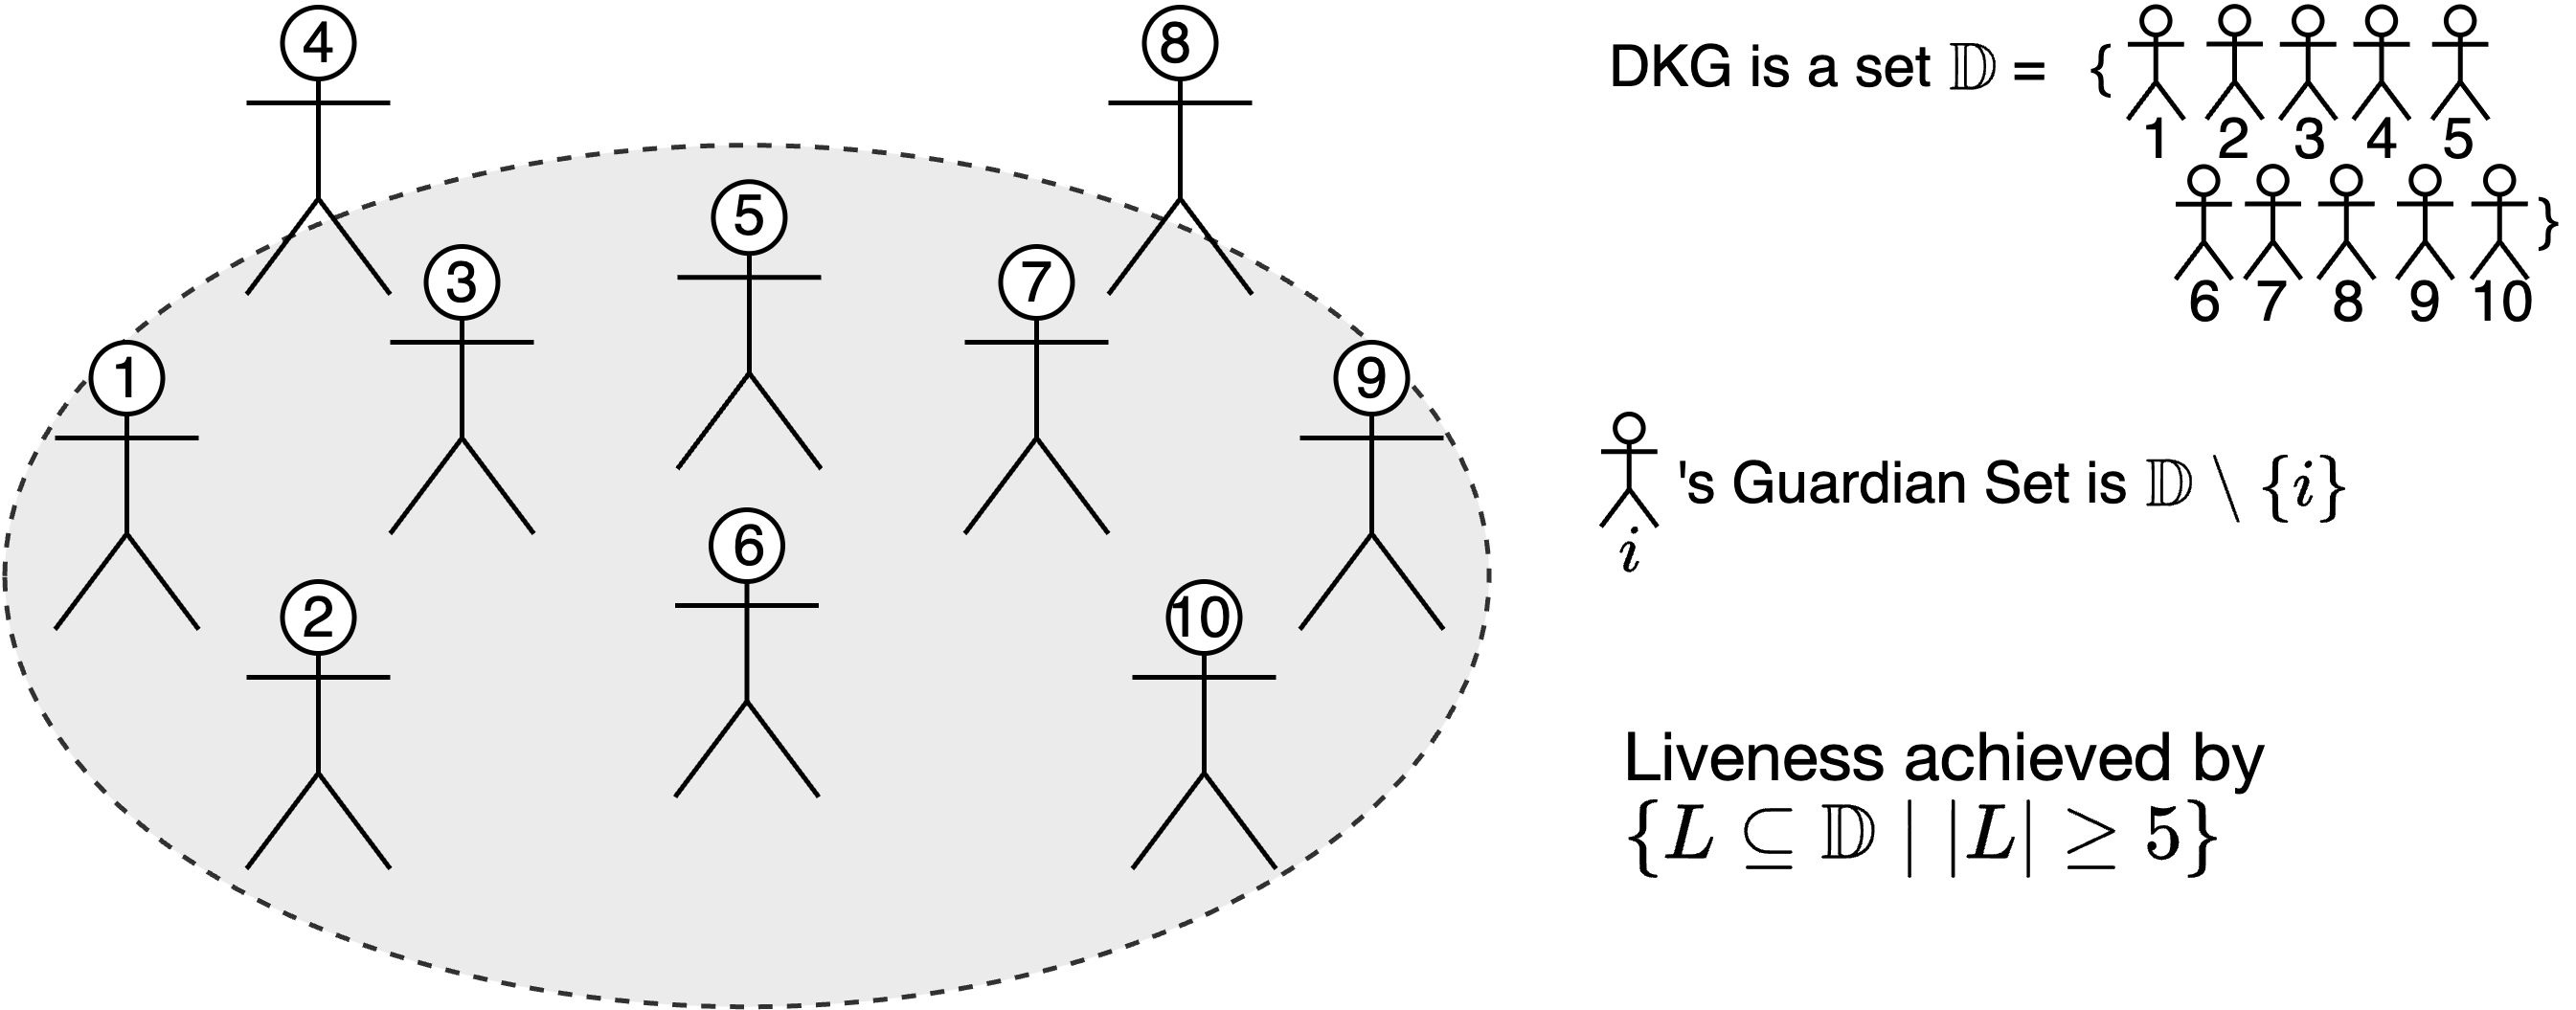
\includegraphics[width=.5\textwidth]{DKG-example.png} \\
    \vspace{0.5em} 
    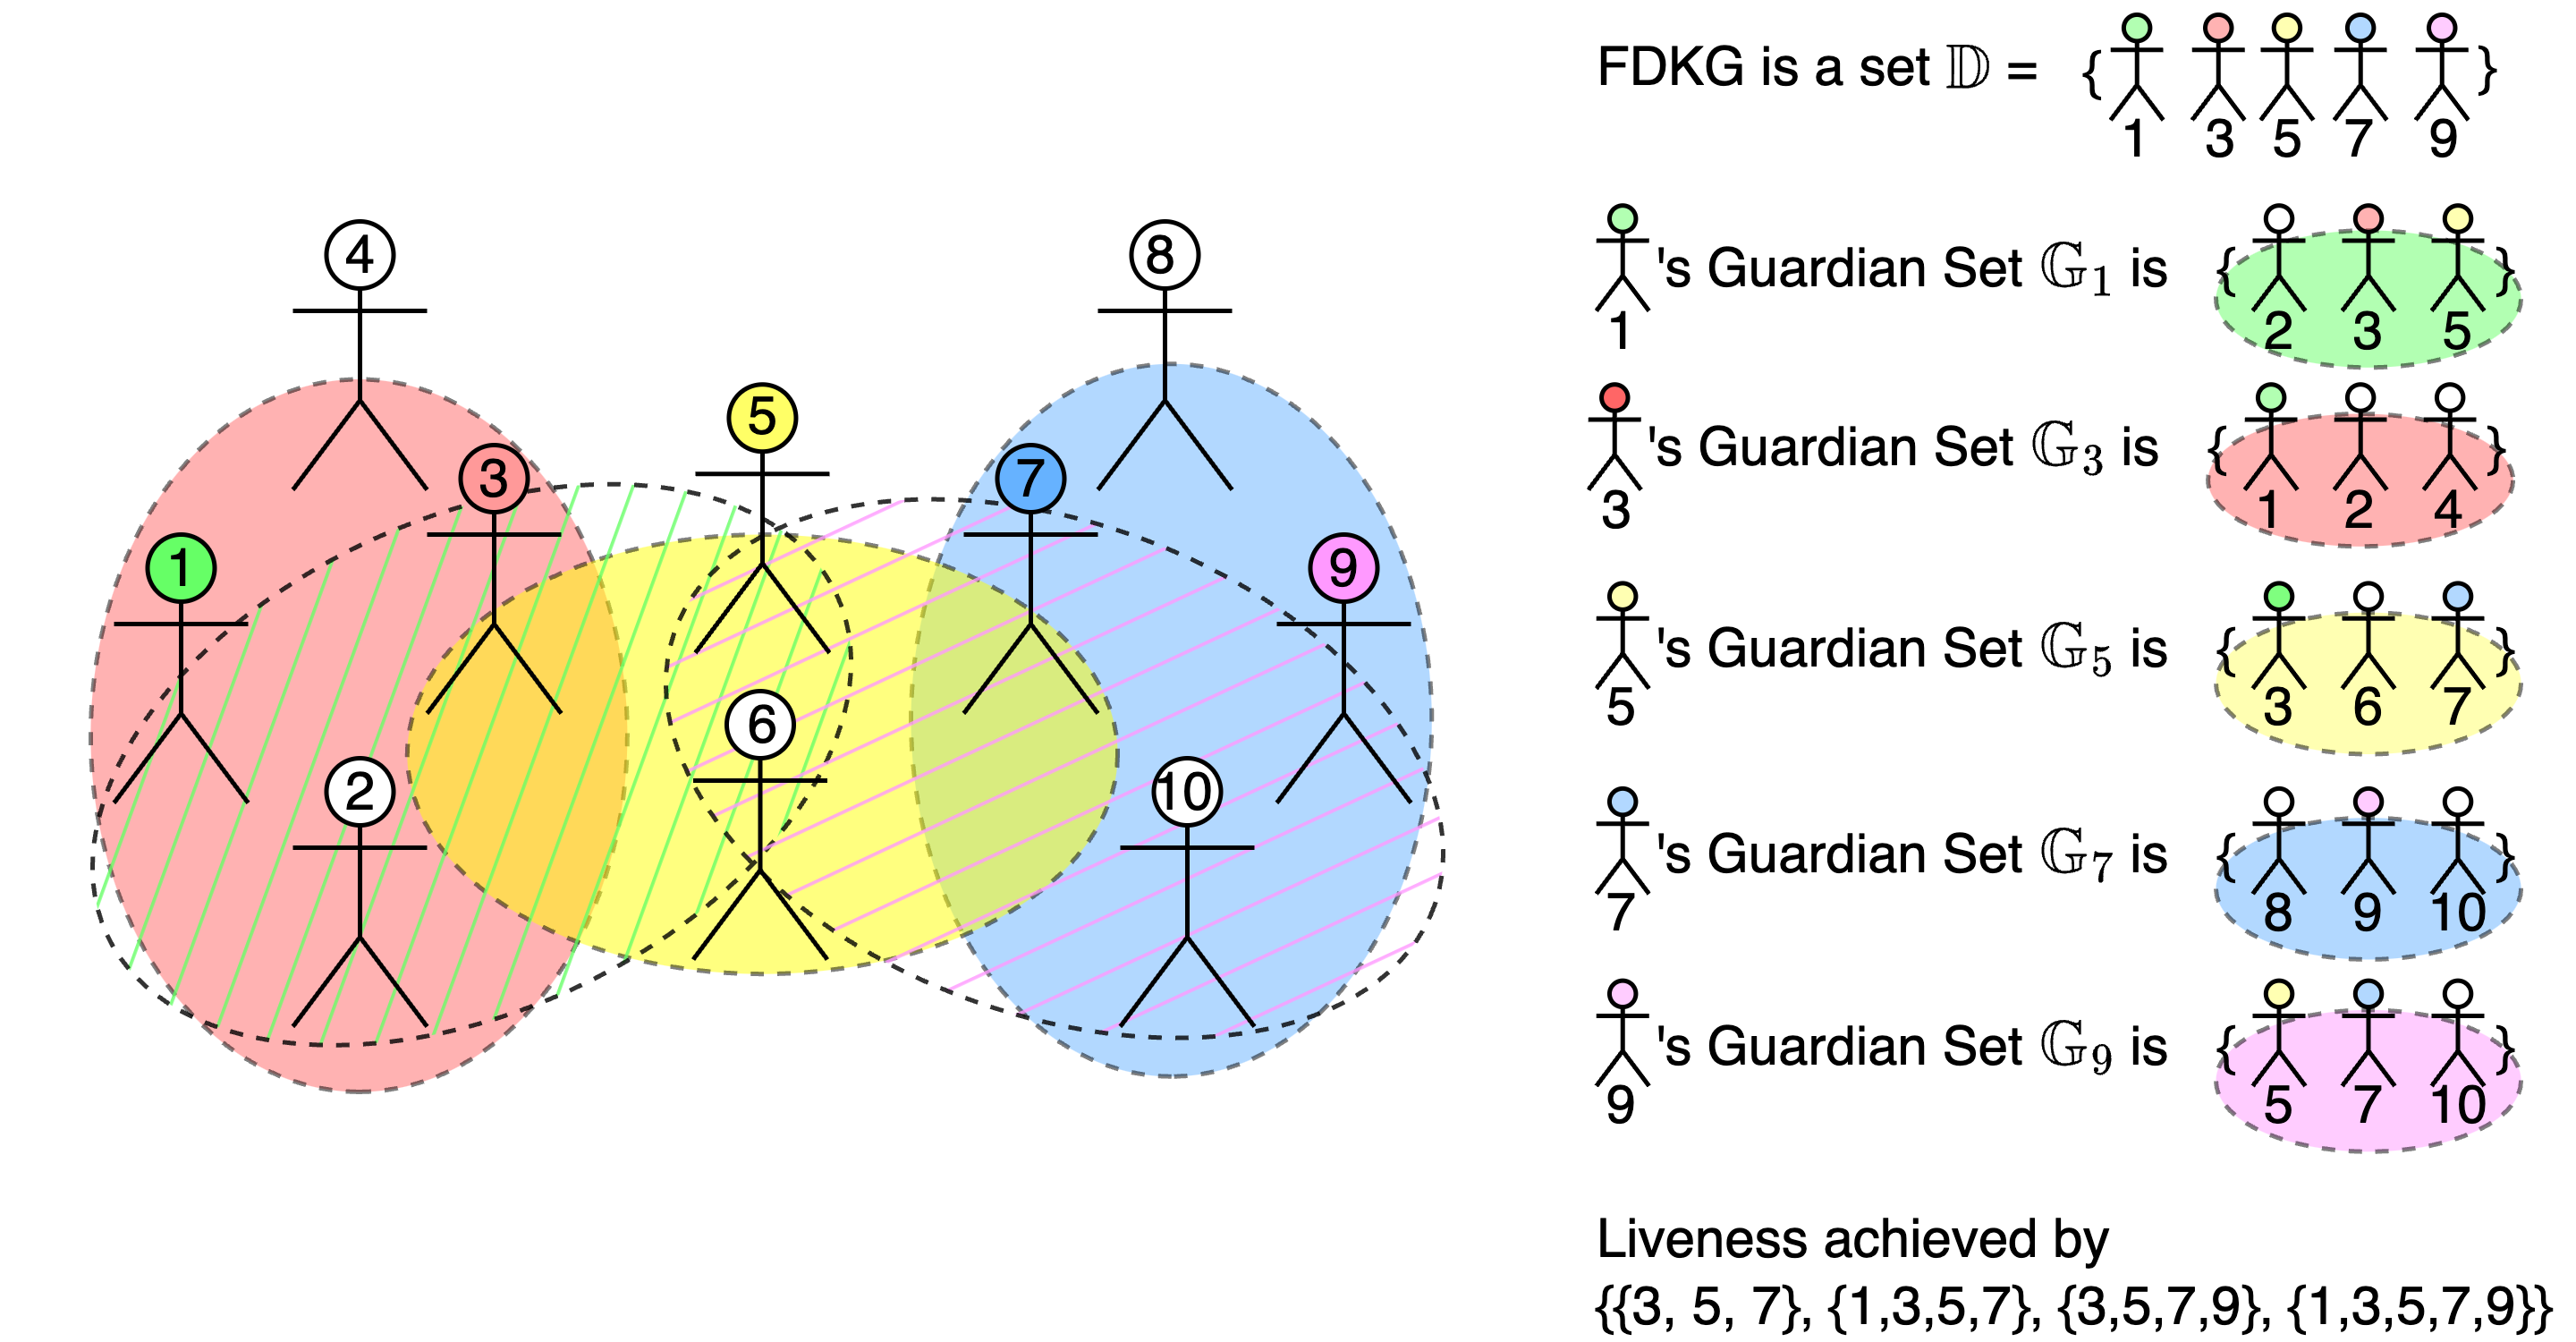
\includegraphics[width=.5\textwidth]{FDKG-example.png}
    \caption{Visual comparison of $(10,5)$-DKG protocol (above) and $(10, 0.5, 2, 3)$-FDKG (below)}
    \label{fig:FDKG}
\end{figure}

The FDKG process for each participant is as follows:

\begin{enumerate}
    \item \textbf{Party $P_1$}:
        \begin{itemize}
            \item Chooses Guardian Set $\mathbb{G}_1 = \{P_2, P_3, P_5\}$.
            \item Samples a random polynomial $f_1(X) \in_R \mathbb{Z}_q[X]$, computes decryption key $d_1 = f_1(0)$.
            \item Distributes $d_1$ among $\mathbb{G}_1$, yielding shares $\SharePartialSecretKey{1}{2}, \SharePartialSecretKey{1}{3}, \SharePartialSecretKey{1}{5}$.
        \end{itemize}

    \item \textbf{Party $P_3$}:
        \begin{itemize}
            \item Chooses $\mathbb{G}_3 = \{P_1, P_2, P_4\}$.
            \item Samples $f_3(X)$, computes $d_3$, and distributes it among $\mathbb{G}_3$, yielding shares $\SharePartialSecretKey{3}{1}, \SharePartialSecretKey{3}{2}, \SharePartialSecretKey{3}{4}$.
        \end{itemize}

    \item \textbf{Party $P_5$}:
        \begin{itemize}
            \item Chooses $\mathbb{G}_5 = \{P_3, P_6, P_7\}$.
            \item Samples $f_5(X)$, computes $d_5$, and distributes it among $\mathbb{G}_5$, yielding shares $\SharePartialSecretKey{5}{3}, \SharePartialSecretKey{5}{6}, \SharePartialSecretKey{5}{7}$.
        \end{itemize}

    \item \textbf{Party $P_7$}:
        \begin{itemize}
            \item Chooses $\mathbb{G}_7 = \{P_8, P_9, P_{10}\}$.
            \item Samples $f_7(X)$, computes $d_7$, and distributes it among $\mathbb{G}_7$, yielding shares $\SharePartialSecretKey{7}{8}, \SharePartialSecretKey{7}{9}, \SharePartialSecretKey{7}{10}$.
        \end{itemize}

    \item \textbf{Party $P_9$}:
        \begin{itemize}
            \item Chooses $\mathbb{G}_9 = \{P_5, P_7, P_{10}\}$.
            \item Samples $f_9(X)$, computes $d_9$, and distributes it among $\mathbb{G}_9$, yielding shares $\SharePartialSecretKey{9}{5},\SharePartialSecretKey{9}{7}, \SharePartialSecretKey{9}{10}$.
        \end{itemize}
\end{enumerate}

In a traditional DKG protocol, the minimum set of parties required to achieve Liveness (Definition~\ref{def:liveness}) would be any subset of size at least $t$ e.g., \(\{P_1, P_3, P_5, P_7, P_9 \}\). However, with the FDKG approach, the use of dynamic Guardian Sets and therefore emergent significance factor of parties, this minimum set can be reduced to $\{P_3, P_5, P_7\}$, demonstrating the protocol's efficiency in reducing the number of participants required for successful deconstruction.

\section{Security Properties}
\label{sec:security_properties}

This section formalizes the security guarantees of the FDKG protocol. We define three core properties---\textbf{Liveness}, \textbf{Integrity}, and \textbf{Privacy}---that address distinct adversarial threats and resilience objectives. Each property operates at a different scope:
\begin{itemize}
    \item \textbf{Liveness} ensures network-wide key reconstruction despite partial failures or adversarial interference.
    \item \textbf{Privacy} protects individual participants' partial secret keys from unauthorized disclosure.
    \item \textbf{Integrity} guarantees cryptographic consistency and correctness of the reconstructed global secret key.
\end{itemize}

\subsection{Liveness}
\label{subsec:liveness}

\textbf{Liveness} in FDKG ensures that the global secret key \(\SecretKey = \sum \PartialSecretKey{i}\) can be reconstructed from the shares of honest participants and their guardians, even in the presence of adversarial interference or node failures.

\begin{definition}[Liveness]
\label{def:liveness}
The FDKG protocol achieves \textbf{Liveness} if, for every participant \(\Party{i} \in \mathbb{D}\), either:
\begin{itemize}
    \item \(\Party{i}\) is honest and publishes its partial secret key \(\PartialSecretKey{i}\), or
    \item At least \(t\) honest guardians in \(\GuardianSetOf{i}\) publish their shares \(\SharePartialSecretKey{i}{j}\), allowing reconstruction of \(\PartialSecretKey{i}\).
\end{itemize}
\end{definition}

Liveness is violated if there exists a \( P_i \in \mathbb{D} \) such that the adversary controls both \( P_i \) (preventing publication of \( \PartialSecretKey{i} \)) and at least \( k - t + 1 \) guardians in \( \GuardianSetOf{i} \) (preventing reconstruction by guardians).

\begin{theorem}[Liveness]
\label{thm:liveness}
The FDKG protocol achieves Liveness if, for every participant \( P_i \in \mathbb{D} \), the adversary does not control both \( P_i \) and \( k - t + 1 \) guardians in \( \GuardianSetOf{i} \).
\end{theorem}

\begin{proof}[Sketch of Proof]
For each participant \(\Party{i} \in \mathbb{D}\):
\begin{itemize}
    \item If \( P_i \) is honest, it publishes \( \PartialSecretKey{i} \), ensuring its contribution to \( \SecretKey \), regardless of guardian control (since \( k - t + 1 \leq k \)).  
    \item If \( P_i \) is corrupt, reconstruction depends on \( \GuardianSetOf{i} \). If the adversary controls fewer than \( k - t + 1 \) guardians, at least \( k - (k - t) = t \) guardians are honest, ensuring reconstruction via Lagrange interpolation.
\end{itemize}

The condition that the adversary does not control both \(\Party{i}\) and \(k - t + 1\) guardians prevents the adversary from blocking reconstruction by withholding \(\PartialSecretKey{i}\) and corrupting guardians. Thus, \(\SecretKey = \sum \PartialSecretKey{i}\) is recoverable.
\end{proof}

\subsection{Privacy}
\label{subsec:privacy}

\textbf{Privacy} ensures that an adversary cannot learn a participant's partial secret key \(\PartialSecretKey{i}\) unless they control \(\Party{i}\) or a sufficient number of guardians in \(\GuardianSetOf{i}\).

\begin{definition}[Privacy]
\label{def:privacy}
The FDKG protocol ensures \textbf{Privacy} if, for each participant \(\Party{i} \in \mathbb{D}\), an adversary controlling fewer than \(t\) nodes in \(\GuardianSetOf{i}\) and not controlling \(\Party{i}\) learns no information about \(\PartialSecretKey{i}\). Privacy is violated if the adversary either:
\begin{itemize}
    \item Controls \(\Party{i}\), who knows \(\PartialSecretKey{i}\), or
    \item Controls at least \(t\) guardians in \(\GuardianSetOf{i}\), allowing reconstruction of \(\PartialSecretKey{i}\).
\end{itemize}
\end{definition}

\begin{theorem}[Privacy]
\label{thm:privacy}
The FDKG protocol achieves Privacy under the security of the encryption scheme and the properties of Shamir's Secret Sharing.
\end{theorem}

\begin{proof}[Sketch of Proof]
Each share \(\SharePartialSecretKey{i}{j}\) is encrypted using \(\Party{j}\)'s public key, ensuring that only \(\Party{j}\) can decrypt it. Furthermore, by the properties of Shamir's Secret Sharing, any subset of fewer than \(t\) shares reveals no information about \(\PartialSecretKey{i}\). Thus, an adversary controlling fewer than \(t\) guardians learns nothing about \(\PartialSecretKey{i}\), and controlling \(\Party{i}\) directly reveals \(\PartialSecretKey{i}\).
\end{proof}

\subsection{Integrity}
\label{subsec:integrity}

\textbf{Integrity} ensures that the reconstructed global secret key \(\SecretKey\) is consistent with the sum of valid partial secret keys, even in the presence of adversarial interference, provided that all proofs verify.

\begin{definition}[Integrity]
\label{def:integrity}
Let \(\mathbb{H} \subseteq \mathbb{D}\) denote the set of honest parties. \textbf{Integrity} holds if, in an adversarial context where all proofs (\(\ProofFDKG{i}\), \(\ProofPS{i}\), \(\ProofSPS{j}{i}\)) verify, the reconstructed global secret key is:
\[
\SecretKey{} = \sum_{\Party{i} \in \mathbb{H}} \PartialSecretKey{i} + \sum_{\Party{j} \in \mathbb{D} \setminus \mathbb{H}} \widetilde{\PartialSecretKey{j}},
\]
where \(\widetilde{\PartialSecretKey{j}}\) is either \(\PartialSecretKey{j}\) (if recovered) or \(0\) (if blocked or redundant).
\end{definition}

\begin{theorem}[Integrity]
\label{thm:integrity}
The FDKG protocol achieves Integrity if all proofs (\(\ProofFDKG{i}\), \(\ProofPS{i}\), \(\ProofSPS{j}{i}\)) verify.
\end{theorem}

\begin{proof}[Sketch of Proof]
By Definition \ref{def:integrity}, Integrity requires that \(\SecretKey{}\) equals the sum of valid partial secrets. This holds because:
\begin{enumerate}
    \item For honest participants \(\Party{i} \in \mathbb{H}\), \(\ProofFDKG{i}\) ensures that \(\PartialPublicKey{i} = \PartialSecretKey{i} G\) and that the encrypted shares \(\EncryptedSharePartialSecretKey{i}{j}\) are correctly generated from a polynomial \(f_i(X)\) with \(f_i(0) = \PartialSecretKey{i}\).
    \item For potentially corrupt participants \(\Party{j} \in \mathbb{D} \setminus \mathbb{H}\), if \(\PartialSecretKey{j}\) is recovered (either directly via \(\ProofPS{j}\) or through reconstruction from shares with \(\ProofSPS{j}{i}\)), it is consistent with \(\PartialPublicKey{j}\).
    \item If \(\PartialSecretKey{j}\) cannot be recovered due to adversarial blocking, it is effectively set to \(0\), ensuring that \(\SecretKey{}\) remains the sum of the recoverable partial secrets.
\end{enumerate}
Thus, by the soundness of the zk-SNARKs and the properties of Publicly Verifiable Secret Sharing (PVSS), the reconstructed \(\SecretKey{}\) is consistent with the sum of valid partial secrets.
\end{proof}

% \section{Security Properties}
% \label{sec:security_properties}

% This section formalizes the security guarantees of the FDKG protocol. We define three core properties—Liveness, Privacy, Integrity—that address distinct adversarial threats and resilience objectives. Each property operates at a different scope:
% \begin{itemize}
%     \item \textbf{Local Safety} focuses on preventing unrecoverability via local collusion in a single guardian set.
%     \item \textbf{Global Liveness} focuses on ensuring recoverability despite global faults across the network.
%     \item \textbf{Correctness} guarantees cryptographic consistency and integrity of the reconstructed secret.
% \end{itemize}

% \subsection{Local Safety}
% \label{subsec:local-safety}

% Local Safety operates at the \textit{per-guardian-set} level. Its goal is to prevent adversaries from blocking reconstruction of a specific participant’s share through targeted collusion.  

% \begin{definition}[Local Safety]
% \label{def:local-safety}
%     Local Safety is violated if there exists a party $\Party{i} \in \mathbb{D}$ such that the adversary controls both $\Party{i}$ itself, and at least $k - t + 1$ nodes in $\GuardianSetOf{i}$.
%     Local Safety holds if no such collusion exists.
% \end{definition}

% Each $\GuardianSetOf{i}$ uses a $t$-out-of-$k$ scheme. To reconstruct $\PartialSecretKey{i}$, at least $t$ honest guardians must collaborate.
% Proofs $\ProofFDKG{i}$ enforce that shares derive from a valid polynomial $f_i(X)$, preventing adversarial manipulation of shares.

% \paragraph{Proof Sketch}  
% Assume Local Safety is violated. The adversary controls $\Party{i}$ and $k - t + 1$ guardians in $\GuardianSetOf{i}$. Since reconstruction requires $t$ shares, the remaining $t - 1$ honest guardians cannot recover $\PartialSecretKey{i}$, and $\Party{i}$ withholds its share. Thus, $\SecretKey{}$ is unrecoverable. Conversely, if no such collusion exists, all shares are reconstructible.  

% % ---

% \subsection{Global Liveness}
% \label{subsec:global-liveness}

% Global Liveness operates at the \textit{network-wide} level. Its goal is to ensure eventual key reconstruction despite partial failures (e.g., crashes, network partitions).  

% \begin{definition}[Global Liveness]
% \label{def:global-liveness}
%     Global Liveness is achieved if, for every $\Party{i} \in \mathbb{D}$, either:
%     \begin{itemize}
%         \item $\Party{i}$ is honest and publishes $\PartialSecretKey{i}$, or
%         \item At least $t$ nodes in $\GuardianSetOf{i}$ are honest and publish $\SharePartialSecretKey{i}{j}$.
%     \end{itemize}
% \end{definition}

% Each $\GuardianSetOf{i}$ contains $k$ nodes, ensuring at least $t$ remain honest if $k - t$ are corrupt.
% Any party can compute $\SecretKey{}$ using published shares, ensuring recoverability even if participants go offline.
    
% \paragraph{Proof Sketch}  
% For each $\Party{i} \in \mathbb{D}$:  
% \begin{itemize}
%     \item If $\Party{i}$ is honest, $\PartialSecretKey{i}$ is published.
%     \item If $\Party{i}$ is corrupt, by Global Liveness, at least $t$ honest guardians in $\GuardianSetOf{i}$ can reconstruct $\PartialSecretKey{i}$.
% \end{itemize}

% Summing all $\PartialSecretKey{i}$ yields $\SecretKey{}$.  

% \subsection{Liveness}
% \label{subsec:liveness}

% \textbf{Liveness} in FDKG ensures that the global secret key \(\SecretKey = \sum \PartialSecretKey{i}\) can be reconstructed from the shares of honest participants and their guardians, even in the presence of adversarial interference or node failures.

% \begin{definition}[Liveness]
% \label{def:liveness}
% The FDKG protocol achieves \textbf{Liveness} if, for every participant \(\Party{i} \in \mathbb{D}\), either:
% \begin{itemize}
%     \item \(\Party{i}\) is honest and publishes its partial secret key \(\PartialSecretKey{i}\), or
%     \item At least \(t\) honest guardians in \(\GuardianSetOf{i}\) publish their shares \(\SharePartialSecretKey{i}{j}\), allowing reconstruction of \(\PartialSecretKey{i}\).
% \end{itemize}
% \end{definition}

% Liveness can be compromised by an adversary through two primary strategies:
% \begin{enumerate}
%     \item \textbf{Local Attack}: The adversary controls both the participant \(\Party{i}\) and at least \(k - t + 1\) guardians in \(\GuardianSetOf{i}\), preventing the reconstruction of \(\PartialSecretKey{i}\).
%     \item \textbf{Global Attack}: The adversary controls more than \(k - t\) guardians in one or more guardian sets, reducing the number of honest guardians below the threshold \(t\) needed for reconstruction.
% \end{enumerate}

% \subsection{Integrity}
% \label{subsec:integrity}

% Correctness ensures cryptographic consistency across the protocol. Its goal is to guarantee that the reconstructed $\SecretKey{}$ matches the sum of valid partial secrets. 

% \begin{definition}[Integrity]
% \label{def:integrity}
% Let \(\mathbb{H} \subseteq \mathbb{D}\) denote the set of honest parties. \textbf{Integrity} holds if, in an adversarial context where all proofs (\(\ProofFDKG{i}\), \(\ProofPS{i}\), \(\ProofSPS{j}{i}\)) verify, the reconstructed global secret key is:
% \[
% \SecretKey{} = \sum_{\Party{i} \in \mathbb{H}} \PartialSecretKey{i} + \sum_{\Party{j} \in \mathbb{D} \setminus \mathbb{H}} \widetilde{\PartialSecretKey{j}},
% \]
% where \(\widetilde{\PartialSecretKey{j}}\) is either \(\PartialSecretKey{j}\) (if recovered) or \(0\) (if blocked or redundant).
% \end{definition}


% % \begin{definition}[Correctness]
% % \label{def:correctness}
% %     Let $\mathbb{H} \subseteq \mathbb{D}$ denote the set of honest parties. Correctness holds if:
% %     \[
% %     \SecretKey{} = \sum_{\Party{i} \in \mathbb{H}} \PartialSecretKey{i} + \sum_{\Party{j} \in \mathbb{D} \setminus \mathbb{H}} \widetilde{\PartialSecretKey{j}},
% %     \]
% %     where $\widetilde{\PartialSecretKey{j}}$ is either $\PartialSecretKey{j}$ (if recovered) or $0$ (if blocked or redundant).
% % \end{definition}
 
% PVSS Verification enforces that shares $\SharePartialSecretKey{i}{j}$ lie on a degree $t-1$ polynomial $f_i(X)$.
% zkSNARKs enforces that a) $\ProofFDKG{i}$ binds $\EncryptedSharePartialSecretKey{i}{j}$ to $f_i(X)$; b) $\ProofPS{i}$ proves knowledge of $\PartialSecretKey{i}$ for $\PartialPublicKey{i}$; c) $\ProofSPS{j}{i}$ ensures correct decryption of shares. 

% \subsection{Privacy}
% \label{subsec:privacy}

% \textbf{Privacy} ensures that an adversary cannot learn a participant's partial secret key \(\PartialSecretKey{i}\) unless they control \(\Party{i}\) or a sufficient number of guardians in \(\GuardianSetOf{i}\).

% \begin{definition}[Privacy]
% \label{def:privacy}
% The FDKG protocol ensures \textbf{Privacy} if, for each participant \(\Party{i} \in \mathbb{D}\), an adversary controlling fewer than \(t\) nodes in \(\GuardianSetOf{i}\) and not controlling \(\Party{i}\) learns no information about \(\PartialSecretKey{i}\). Privacy is violated if the adversary either:
% \begin{itemize}
%     \item Controls \(\Party{i}\), who knows \(\PartialSecretKey{i}\), or
%     \item Controls at least \(t\) guardians in \(\GuardianSetOf{i}\), allowing reconstruction of \(\PartialSecretKey{i}\).
% \end{itemize}
% \end{definition}



% \subsection{Security Theorems}
% \label{subsec:security-theorems}

% Local Safety addresses stronger adversarial power ($k - t + 2$ nodes) but focuses on single guardian sets. Global Liveness addresses weaker adversarial power ($k - t$ nodes) but applies network-wide.

% If the adversary controls $k - t + 1$ nodes in every guardian set (violating Global Liveness), they still cannot violate Local Safety unless they also control the participant ($k - t + 2$ nodes total). Conversely, if the adversary controls $k - t + 2$ nodes in a guardian set (violating Local Safety), they automatically violate Global Liveness for that set.  

% \begin{theorem}[Local Safety]
% \label{thm:local-safety}
%     The FDKG protocol achieves Local Safety if, for every guardian set $\GuardianSetOf{i}$, the adversary controls fewer than $k - t + 2$ nodes (i.e., the participant $\Party{i}$ and fewer than $k - t + 1$ guardians).
% \end{theorem}

% \begin{proof}
%     By Definition~\ref{def:local-safety}, violating Local Safety requires controlling $\Party{i}$ and $k - t + 1$ guardians. If the adversary controls fewer than $k - t + 1$ guardians in every $\GuardianSetOf{i}$, honest guardians retain a majority ($\geq t$) and can reconstruct $\PartialSecretKey{i}$.
% \end{proof}

% \begin{theorem}[Global Liveness]
% \label{thm:global-liveness}
%     The FDKG protocol achieves Global Liveness if, for every guardian set $\GuardianSetOf{i}$, the adversary controls at most $k - t$ nodes.
% \end{theorem}

% \begin{proof}
%     If the adversary controls $\leq k - t$ nodes in every $\GuardianSetOf{i}$, at least $t$ honest guardians remain in each set. By the $t$-out-of-$k$ threshold, these guardians can reconstruct $\PartialSecretKey{i}$ for all $\Party{i} \in \mathbb{D}$, ensuring $\SecretKey{}$ is recoverable.
% \end{proof}


% \begin{theorem}[Privacy]
% \label{thm:privacy}
% The FDKG protocol achieves Privacy under the security of the encryption scheme and the properties of Shamir's Secret Sharing.
% \end{theorem}

% \begin{proof}
% Each share \(\SharePartialSecretKey{i}{j}\) is encrypted using \(\Party{j}\)'s public key, ensuring that only \(\Party{j}\) can decrypt it. Furthermore, by the properties of Shamir's Secret Sharing, any subset of fewer than \(t\) shares reveals no information about \(\PartialSecretKey{i}\). Thus, an adversary controlling fewer than \(t\) guardians learns nothing about \(\PartialSecretKey{i}\), and controlling \(\Party{i}\) directly reveals \(\PartialSecretKey{i}\).
% \end{proof}

% \begin{theorem}[Integrity]
% \label{thm:integrity}
% The FDKG protocol achieves \textbf{Integrity} if all proofs (\(\ProofFDKG{i}\), \(\ProofPS{i}\), \(\ProofSPS{j}{i}\)) verify.
% \end{theorem}

% \paragraph{Proof Sketch}
% By Definition~\ref{def:integrity}, Integrity requires that \(\SecretKey{}\) equals the sum of valid partial secrets, even in the presence of adversaries, provided that all zk-SNARK proofs verify. This holds because:
% \begin{enumerate}
%     \item For honest participants \(\Party{i} \in \mathbb{H}\), \(\ProofFDKG{i}\) ensures that \(\PartialPublicKey{i} = \PartialSecretKey{i} G\) and that the shares \(\EncryptedSharePartialSecretKey{i}{j}\) are correctly encrypted evaluations of a polynomial \(f_i(X)\) with \(f_i(0) = \PartialSecretKey{i}\).
%     \item For potentially corrupt participants \(\Party{j} \in \mathbb{D} \setminus \mathbb{H}\), if \(\PartialSecretKey{j}\) is recovered (via \(\ProofPS{j}\) or reconstruction from shares with \(\ProofSPS{j}{i}\)), it is consistent with \(\PartialPublicKey{j}\).
%     \item If \(\PartialSecretKey{j}\) cannot be recovered due to adversarial blocking, it is effectively set to \(0\), ensuring that \(\SecretKey{}\) remains the sum of recoverable partial secrets.
% \end{enumerate}
% Thus, by the soundness of the zk-SNARKs and the properties of Publicly Verifiable Secret Sharing (PVSS), the reconstructed \(\SecretKey{}\) is consistent with the sum of valid partial secrets.



\section{Liveness Simulations}
\label{sec:liveness_simulations}

To evaluate FDKG's resilience under realistic deployment conditions, we conducted simulations comparing our protocol with traditional DKG implementations. Our analysis focuses on three aspects: 1) parameter sensitivity, 2) scalability across network sizes, and 3) topology-dependent performance characteristics. The primary objective was to determine which configurations optimize liveness under varying conditions, thereby offering insights for practical deployment.

\subsection{Simulation Methodology}
\label{subsec:methodology}

We developed a simulation framework implementing both FDKG and DKG protocols across two network topologies. Each simulation involves the following steps:


\begin{enumerate}
    \item \textbf{Network Generation:} We considered two network topologies to represent real-world communication patterns:
    \begin{itemize}
        \item \textbf{Barabási-Albert (BA):} A scale-free model designed to simulate scenarios where nodes exhibit preferential attachment, creating highly connected hubs.
        \item \textbf{Random Graph:} A uniform model representing scenarios where nodes interact uniformly, with no highly connected hubs.
    \end{itemize}
    
    Networks were initialized with a specified number of nodes ($n$) and average connections per node, governed by the number of guardians ($k$). 
    \item \textbf{Participant Selection:} For each simulation, subsets of nodes were selected to participate in the protocol phases:
    \begin{itemize}
        \item \emph{Distribution Participants:} A proportion $p$ of nodes were randomly selected based on their connectivity (degree in the graph).
        \item \emph{Reconstruction Participants:} Nodes responsible for reconstructing the secret were selected proportionally ($r$) from the Distribution Participants.
    \end{itemize}
    
    \item \textbf{Liveness Check:} For each simulation, the protocol checked whether the remaining talliers could successfully meet the threshold required for reconstructing the secret. Success was defined as achieving \emph{Liveness} (Definition~\ref{def:liveness}) by reconstructing the secret despite node failures or absences.
\end{enumerate}

The web simulator is available at: \url{https://fdkg.stan.bar}, source code is available at \url{https://github.com/stanbar/PeerVote}. Figure~\ref{fig:network_examples} presents a snapshot of two different network topologies for the same setting.

\begin{figure}[h]
    \centering
    \begin{minipage}{0.24\textwidth}
        \centering
        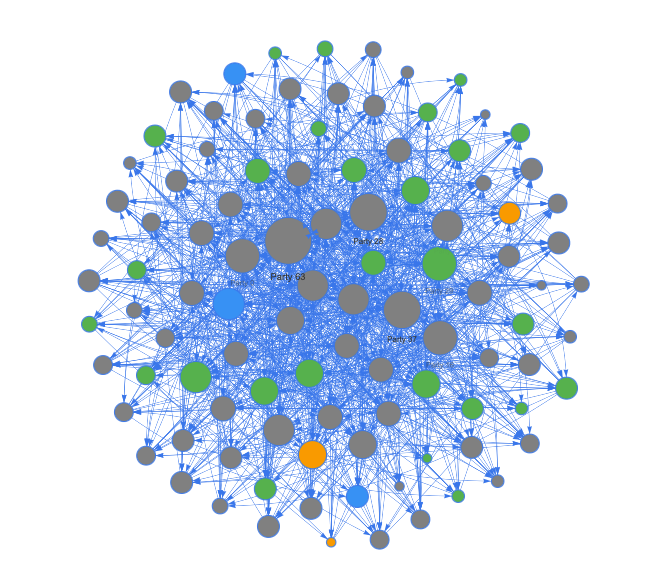
\includegraphics[width=\textwidth]{Random_100nodes_30p_90r_3_of_5.png}
        \label{fig:random_100_30_90_3_5}
    \end{minipage}
    \hfill
    \begin{minipage}{0.24\textwidth}
        \centering
        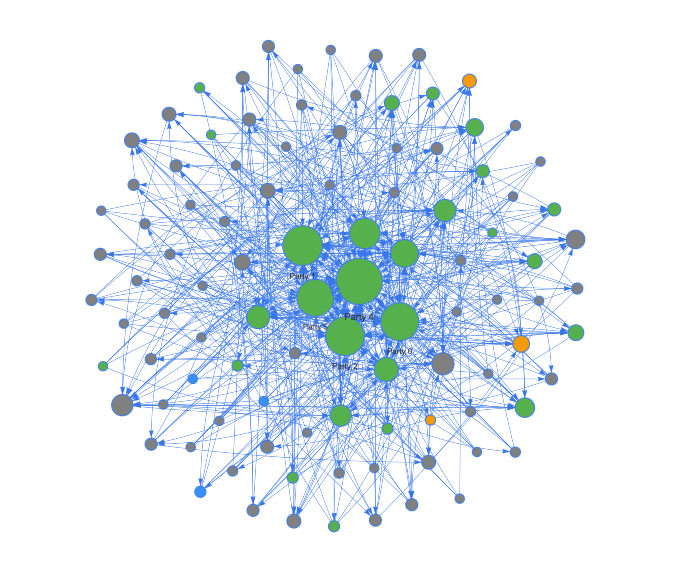
\includegraphics[width=\textwidth]{BA_100nodes_30p_90r_3_of_5.png}
        \label{fig:example_ba_network}
    \end{minipage}
    
    \caption{Comparison of Random (left) and Barabási-Albert (right) guardian set selection policies for $n = 100, p=0.3, r=0.9, k=5, t=3$. Gray nodes indicate the absence of the node, green nodes represent those that were present in both the distribution and reconstruction phases, blue nodes were present only in the first (distribution) phase, and orange nodes only in the second (reconstruction) phase.}
    \label{fig:network_examples}
\end{figure}

\subsection{Parameter Space and Simulation Workflow}

We explored a comprehensive range of parameters to capture diverse deployment scenarios:
\begin{itemize}
    \item \textbf{Number of Participants ($n$)}: 
    $\{50, 100,200,\dots,1000\}$.
    \item \textbf{Participation Rate ($p$)}: $\{0,1, 0.2, \dots, 0.9, 1.0\}$.
    \item \textbf{Retention Rate ($r$)}: $\{0.1,0.2,\dots,1.0\}$.
    \item \textbf{Number of Guardians ($k$)}: $\{1,3,\dots,n-1\}$.
    \item \textbf{Threshold ($t$)}: Takes values from $1$ up to $k$.
\end{itemize}

For each unique combination of parameters, 100 independent simulations were executed, resulting in over 100 million total runs. 

Figure~\ref{fig:network_model} shows the scalability comparison between network models with fixed $p=1.0$, and $r=0.7$. The Y axis (success rate) is a mean value among all the $(k,t)$ configurations. DKG is a special case configuration for FDKG protocol where $p=1.0$ and $k=n-1$, therefore it becomes the upper bound of the mean success rate with a constant value of $r=0.7$. In DKG each node connect to every other note creating a complete graph, so there is no difference between BA and Random policy. BA policy (solid lines) outperform random policy (dashed) through hub resilience.


\begin{figure}[htbp]
    \centering
    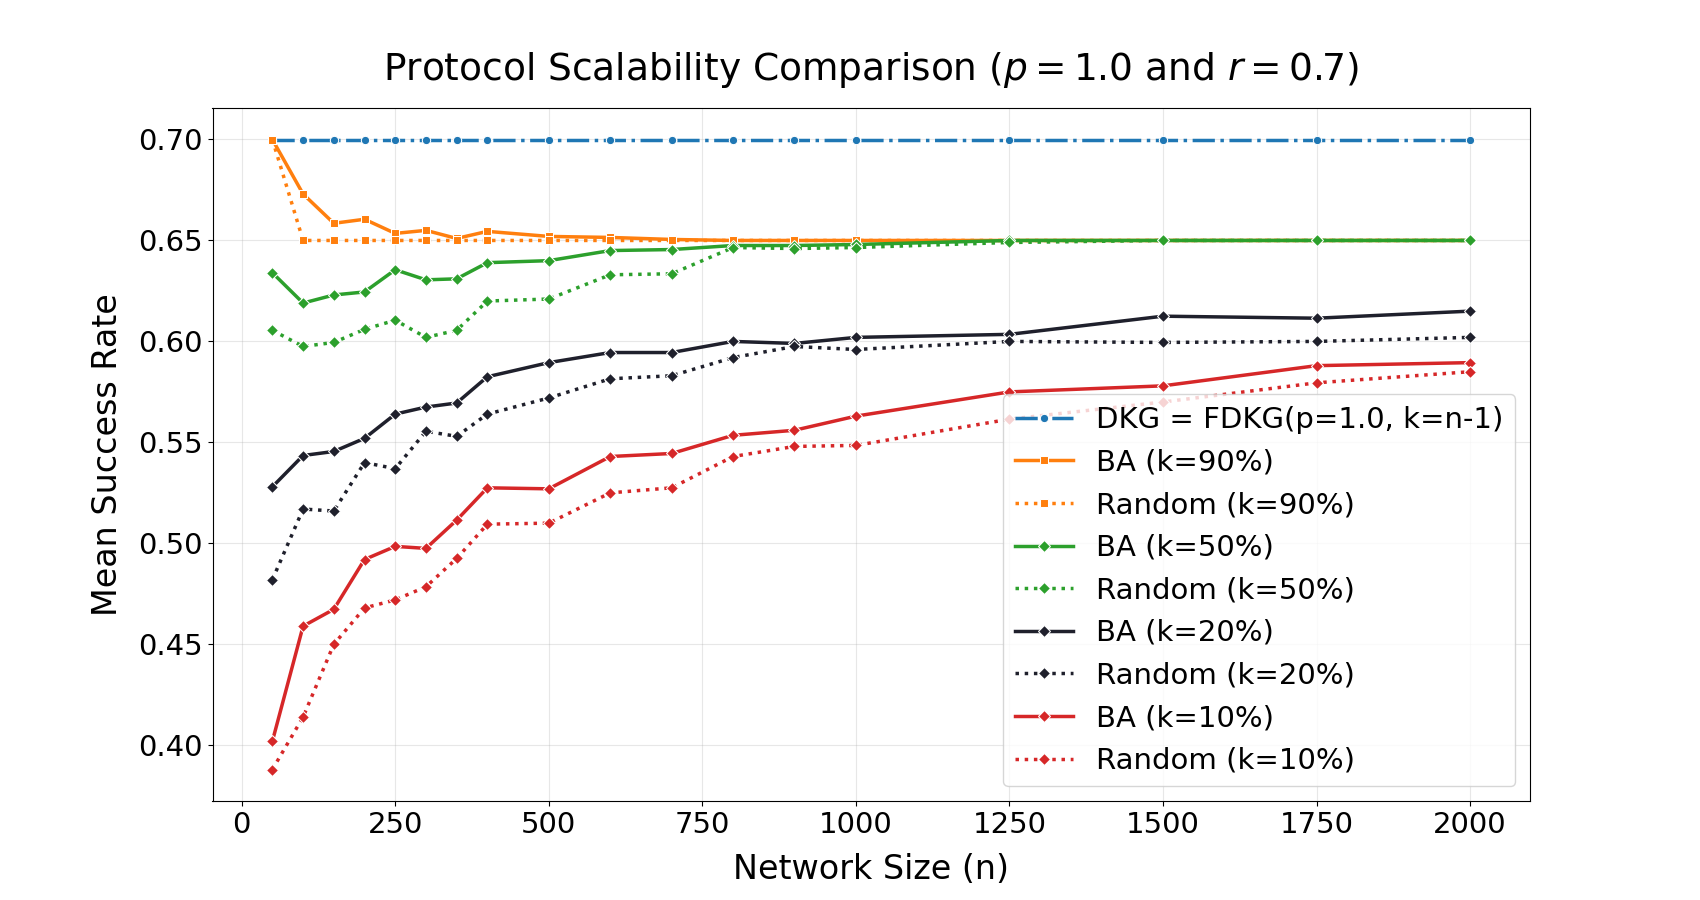
\includegraphics[width=0.5\textwidth]{network_model_comparison.png}
        \caption{Scalability comparison between guardian set size and different policy selection with fixed $p=1.0, r=0.7$. The blue line represent the standard DKG scheme.}
    \label{fig:network_model}
\end{figure}


Then we break down the mean values to see how each parameter influence the success rate. Also, to focus on the rest of the parameters, from now on we use only the results from BA policy selection.

Figures~\ref{fig:guardian_configs} show success rates for each of the $(k,t)$ configurations for fixed $n=100$, $p=0.8$, and Figure a) $r=0.5$ Figure b) $r=0.8$ highlighting the critical significance of the retention $r$ parameter.


\begin{figure}[htbp]
    
        \centering
        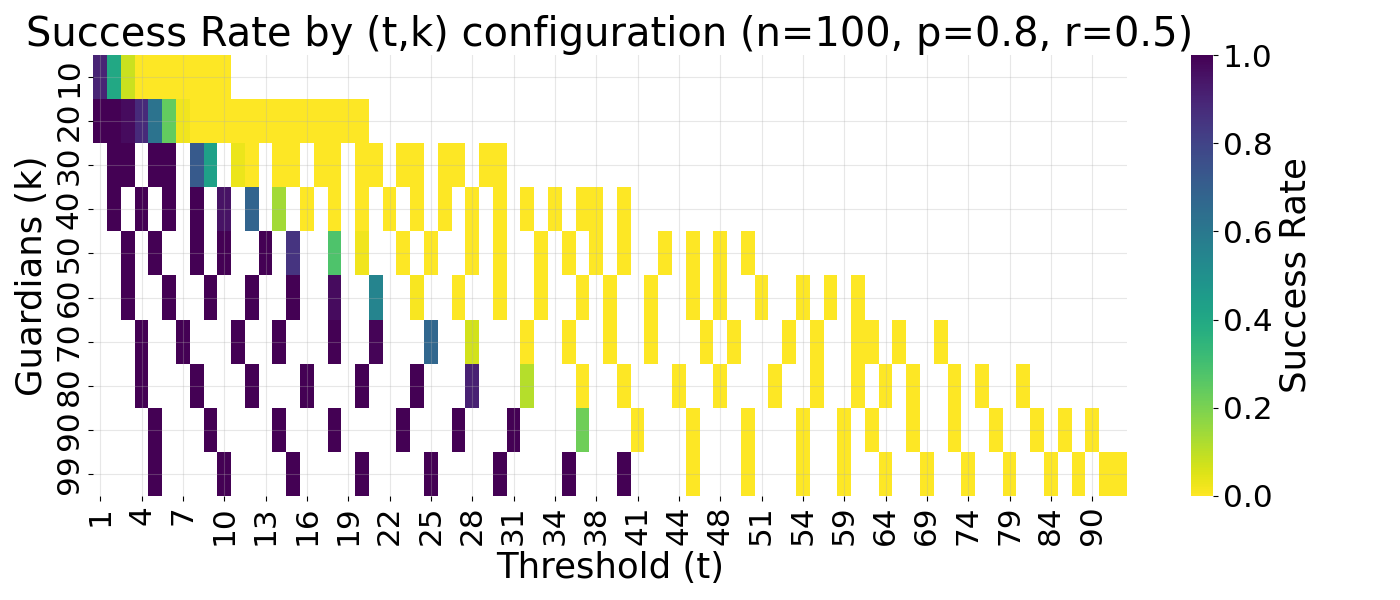
\includegraphics[width=0.48\textwidth]{guardian_set_configuration_n100_p0.8_r0.5.png}
        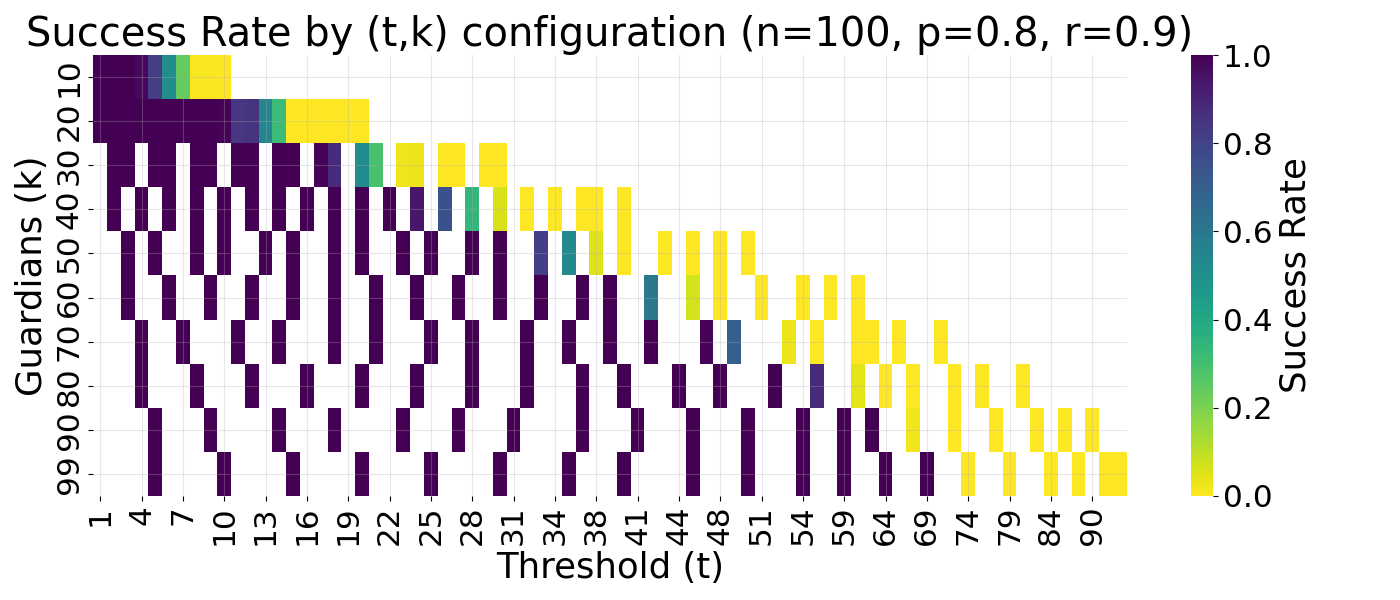
\includegraphics[width=0.48\textwidth]{guardian_set_configuration_n100_p0.8_r0.9.png}
        \label{fig:guardian_set_config_09}

    \caption{Heatmaps of success rates by guardian configuration for fixed $n=100$, $p=0.8$, $r=0.5$ (top) and $r=0.9$ (bottom). Color intensity represents success probability from 0 (yellow) to 1 (dark blue).}
    % TODO: update the captions
    \label{fig:guardian_configs}
\end{figure}


Figures~\ref{fig:parameters_significance_participation} reveal three critical relationships through our multivariate analysis. Higher retention rate $r=0.9$ guarantees success rate even for smaller number of guardians ($k=10$) at partial participation rate $p=0.75$. Lower retention rate $r=0.5$ may require higher participation rate $\geq0.6$ and higher number of guardians $k\geq40$ to achieve perfect success rate. Lower retention rates $\leq0.5$ and low number of guardians $<=10$ may not guarantee success rates even at perfect participation rate $p=1.0$.

\begin{figure}[htbp]
        \centering
        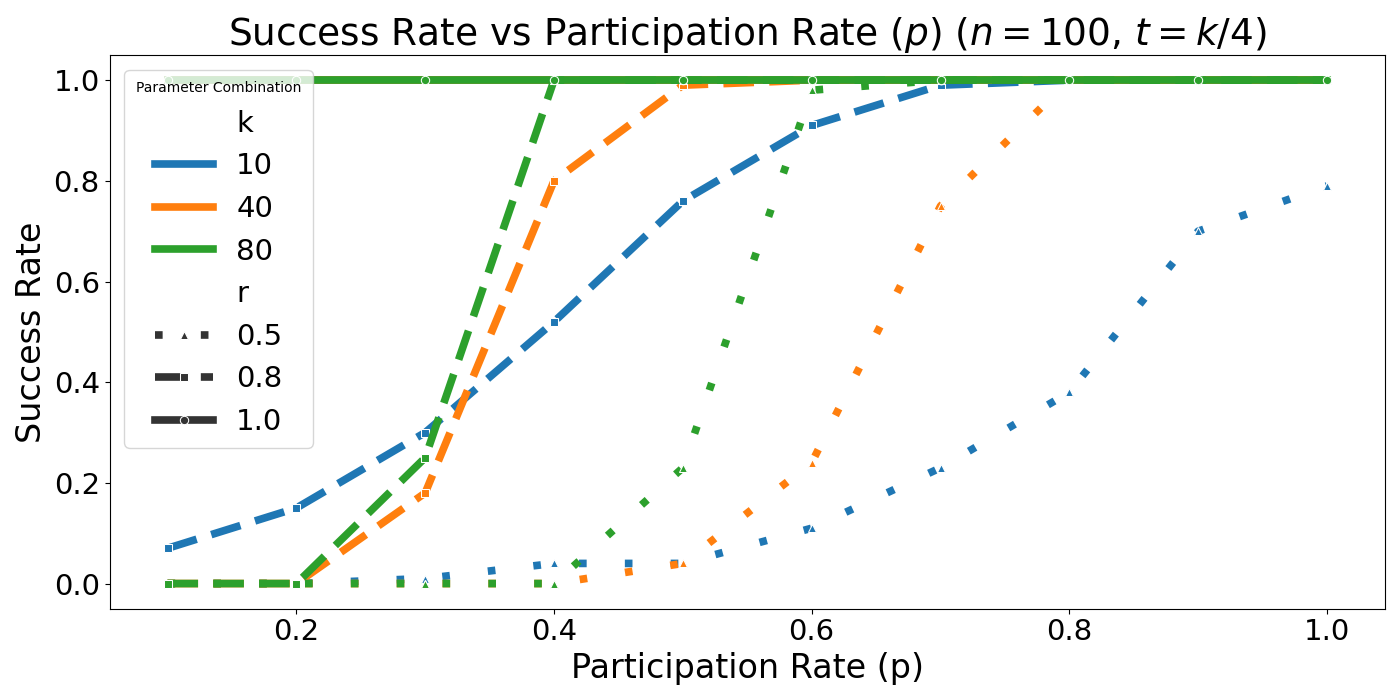
\includegraphics[width=0.5\textwidth]{parameters_significance_participation_axis.png}
        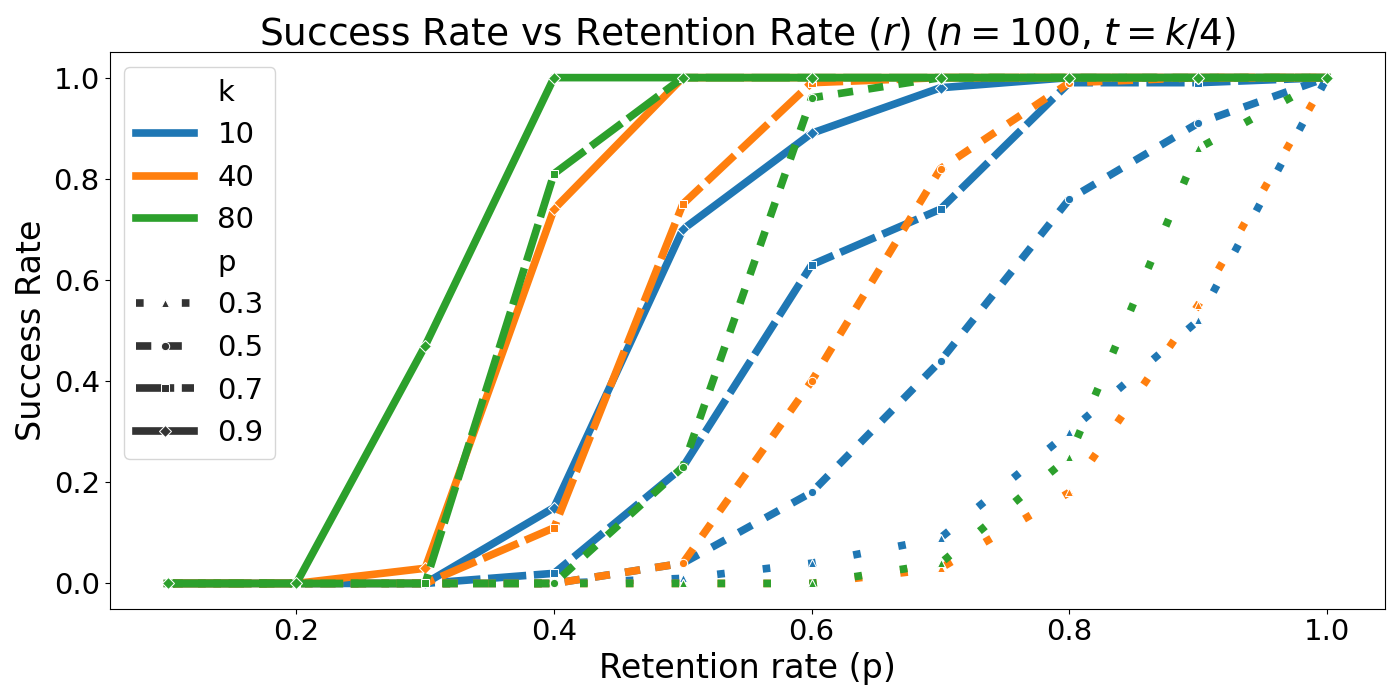
\includegraphics[width=0.5\textwidth]{parameters_significance_retention_axis.png}
        \caption{Success rate vs participation rate (top) and retention rate (bottom) for varying $k$, and $p$, or $r$ combinations, with fixed $n=100$ and $t=k/4$. Line styles represent retention or participation rates, colors indicate guardian set sizes.}
    \label{fig:parameters_significance_participation}
\end{figure}

\subsection{Results}

The results reveal clear trends in the factors influencing success rate. The participation rate ($p$) has a significant impact, with higher participation rates consistently improving success rates. This is because the more nodes that actively participate, the higher the likelihood of meeting the threshold \(t\) during the reconstruction phase.

Retention rate ($r$) also plays a crucial role. Higher retention rates both reduce the reliance on guardians and increase the chances of meeting the threshold during reconstruction phase. For instance, when $r = 1.0$, the protocol always achieves Liveness even with very low participation $p$ and guardians $k$, it is because the party who contributed to the first phase always reconstruct the share in the second phase. However, such scenarios were excluded from the analysis since they do not represent the challenges of FDKG systems.

The number of guardians ($k$) contributes to the robustness of the system, especially in scenarios with a larger total number of nodes. Larger guardian sets provide greater redundancy, mitigating the impact of absent nodes during reconstruction. This becomes increasingly important as the system scales, where the probability of absences rises proportionally with the total number of participants.

Threshold values ($t$) also affect success rates. Lower thresholds are more likely to achieve liveness since fewer nodes are required to reconstruct the secret. However, higher thresholds can still succeed if combined with sufficiently large guardian sets and high participation rates.

The results highlight also the impact of guardians selection policy on liveness, particularly the advantage of the Barabási-Albert model over the Random model. The superior performance of the Barabási-Albert model is primarily due to its weighted selection policy. In this policy, nodes with higher connectivity (hubs) are more likely to be selected as participants in both the Distribution and Reconstruction phases. This approach mirrors real-world social structures where highly connected individuals or entities play a more central role in communication and collaboration. Consequently, these hubs are not only more resilient to failures, but are also more likely to engage in critical democratic processes, such as voting or key reconstruction. However, the results show that with the higher network sizes the difference between those models diminishes.

To assess FDKG’s practical performance under realistic deployment conditions---such as node unavailability, varying participation rates, and network churn---we conducted simulations. These simulations complement the formal security guarantees provided in Section~\ref{sec:security_properties}, which ensure resilience against adversarial attacks under cryptographic assumptions. Importantly, the simulations do not aim to prove security; rather, they illustrate how protocol parameters like participation rate (\(p\)), retention rate (\(r\)), guardian set size (\(k\)), and threshold (\(t\)) impact the likelihood of successful key reconstruction in scenarios with non-adversarial failures (e.g., honest node crashes or dropouts). The results offer practical insights for parameter selection in real-world deployments, where both adversarial and non-adversarial challenges must be considered.

\section{Application: FDKG-Enhanced Voting Protocol}\label{sec:voting_scheme}

% AI improve grammar begin
In this section we present the application of FDKG in a voting protocol. The voting protocol integrates the three-round voting scheme from \cite{schoenmakersLectureNotesCryptographic2018}, the multi-candidate encoding method from \cite{haoAnonymousVotingTworound2010}, and the Federated Distributed Key Generation (FDKG) introduced in this paper. Table~\ref{tab:voting-notations} presents the additional notations used in the FDKG-Enhanced Voting Protocol.
% AI improve grammar end

% Table of Notations
\begin{table}[!t]
\caption{Summary of Additional Notations for FDKG-Enhanced Voting Protocol}
\label{tab:voting-notations}
\begin{tabular}{>{\centering\arraybackslash}p{.25\linewidth}p{.7\linewidth}}
\hline
\textbf{Notation} & \multicolumn{1}{c}{\textbf{Description}} \\

\TotalA     & Sum of the first parts of all the casted ballots, i.e., $\TotalA = \sum_{\Party{i} \in \Voters} \BallotA{i}$ \\

\TotalB     & Sum of the second parts of all the casted ballots, i.e., $\TotalB = \sum_{\Party{i} \in \Voters} \BallotB{i}$ \\


\PartialDecryptionFrom{i}      & Partial decryption from \Party{i}, i.e., $\PartialDecryptionFrom{i} = \PartialSecretKey{i} \TotalA$ \\

\SharePartialDecryptionFromTo{i}{j} & Share of partial decryption, from \Party{i} to \Party{j}, i.e., $\SharePartialDecryptionFromTo{i}{j} = \SharePartialSecretKey{i}{j} \TotalA$ \\

$\Voters \subseteq \Parties$ & Subset of parties participating in the 2. Voting phase  \\

$v_i$             & Encoded vote of \Party{i} \\

$\BlindingFactor{i}$ & One-time random value used for secure ElGamal encryption \\

$\Ballot{i}=(\BallotA{i}, \BallotB{i})$     & Encrypted ballot of participant \Party{i} using ElGamal scheme consisting of $(\BallotA{i}, \BallotB{i})$, where $\BallotA{i}=\BlindingFactor{i} \G$, and $\BallotB{i} = \BlindingFactor{i} \PublicKey{} + \Vote{i} \G$ \\

\hline

\ProofPD{i} & zkSNARK proof of correctness of  \PartialDecryptionFrom{i} \\

\ProofPDS{i}{j} & zkSNARK proof of correctness of \SharePartialDecryptionFromTo{i}{j}  \\

\end{tabular}
\end{table}


Our voting protocol is composed of three rounds: (1) FDKG, where keys are generated (2) Vote Casting, where voters encrypt and cast their votes, and (3) Tallying, where the final results are decrypted and counted.

\subsection{Round 1: Federated Distributed Key Generation (FDKG)}

This round is optional. For each participating party $\Party{i} \in \mathbb{D}$, where $\mathbb{D} \subseteq \Parties$:
\begin{enumerate}
    \item Each party selects a guardian set $\GuardianSetOf{i} \subseteq \Parties \setminus \{\Party{i}\}$.

    \item Each party samples a random polynomial $f_{i}(X) \in_{\$} \mathbb{Z}_q[X]$ of degree $t-1$.
    
    \item  Each party computes its partial secret $\PartialSecretKey{i}= f_i(0)$ and public key $\PartialPublicKey{i} = \PartialSecretKey{i} \G$.
    
    \item  Each party generates shares of the partial secret $\SharePartialSecretKey{i}{j}=f_i(j)$ for each guardian $P_j \in \GuardianSetOf{i}$, which are encrypted using the private channel: $\EncryptedSharePartialSecretKey{i}{j}=\EncryptionUsingOf{\Party{j}}{\SharePartialSecretKey{i}{j}}$.
    \item Each party generates a zero-knowledge proof $\ProofFDKG{i}$, as described in Section~\ref{app:proof-fdkg}.
    \item Each party broadcasts (\PartialPublicKey{i}, \EncryptedSharePartialSecretKey{i}{j}, \ProofFDKG{i}).
\end{enumerate}
\paragraph*{State after Round 1:}
Upon completion of FDKG, the message board contains:
\begin{itemize}
    \item $\{\PartialPublicKey{i} : \Party{i} \in \mathbb{D}\}$, the set of partial encryption keys, where $\PublicKey$ can be reconstructed by anyone by summing $\PublicKey=\sum_{\Party{i} \in \mathbb{D}} \PartialPublicKey{i}$.
    \item $\bigcup_{\Party{i} \in \mathbb{D}} \{C_{i,j} \mid P_j \in \mathbb{G}_i\}$, the set of encrypted shares of the partial decryption keys.
\end{itemize}

\subsection{Round 2: Vote Casting}

For each voter $\Party{i} \in \mathbb{V}$, where $\mathbb{V} \subseteq  \mathbb{P}$:
\begin{enumerate}
     \item Each voter encodes its vote into a scalar value $\Vote{i}$ using the method outlined in \cite{baudronPracticalMulticandidateElection2001}, where votes for each candidate is a power of 2: \[ \Vote{i}\ =\ \begin{cases} 2^0 & \text{if } \Party{i} \text{ votes for candidate 1} \\ 2^m & \text{if } \Party{i} \text{ votes for candidate 2} \\ \vdots & \vdots \\ 2^{(c-1)m} & \text{if } \Party{i} \text{ votes for candidate $c$}\end{cases}\]
where $m$ is the smallest integer such that $2^m > |\Parties|$.
    \item Each voter encrypts their vote by generating a random value $\BlindingFactor{i} \in_{\$} \mathbb{Z}_q$ and producing the ballot: $\Ballot{i} = (\BlindingFactor{i} \G,\ \BlindingFactor{i} \PublicKey{} + \Vote{i} \G)$.
   \item Each voter generates a zero-knowledge proof \ProofBALLOT{i}, as described in Section~\ref{app:proof-ballot}.
    \item Each voter broadcasts $(\Ballot{i}, \ProofBALLOT{i})$.
\end{enumerate}
\paragraph{State after Voting}

After the voting phase concludes, the message board's state is appended with:
\begin{itemize}
    \item $\{\Ballot{i} : \Party{i} \in \Voters\}$, the set of encrypted votes.
\end{itemize}

\subsection{Round 3: Tallying}

The tallying process occurs in two phases: online and offline.

\subsubsection{Online Tally}
A subset of parties $\Tallies \subseteq \Parties$ are involved in a threshold ElGamal decryption. This subset includes at least $t$ parties from each guardian set.
For each party $\Party{i} \in \mathbb{T}$:

\begin{enumerate}
    \item Each party computes the sum of the first component of each ballot $\TotalA = \sum_{\Party{i} \in \mathbb{V}} \BallotA{i}$, where $(\BallotA{i},\BallotB{i})=\Ballot{i}$.
    \item If the party also participated in FDKG ( $\Party{i} \in \SetOfFDKG$):
    \begin{enumerate}
    	\item The party computes the partial decryption $\PartialDecryptionFrom{i} = \PartialSecretKey{i} \TotalA$.
    	\item The party generates a zero-knowledge proof \ProofPD{i} as described in Section~\ref{app:proof-pd}.
    \end{enumerate}
    
    \item For each received encrypted share $\EncryptedSharePartialSecretKey{j}{i}$, where $\Party{j} \in \mathbb{D} \setminus \{\Party{i}\}$ and $\Party{i} \in \GuardianSetOf{j}$:
        \begin{enumerate}
            \item The party decrypts the share and calculates the partial decryption share $\SharePartialSecretKey{j}{i}=\DecryptionUsingOf{\PartySecretKey{i}}{\EncryptedSharePartialSecretKey{j}{i}}$.
            \item The party calculates its share of the partial decryption $\SharePartialDecryptionFromTo{j}{i} = \SharePartialSecretKey{j}{i} \TotalA$.
            \item The party generates a zero-knowledge proof \ProofPDS{j}{i} as described in Section~\ref{app:proof-pds}.
        \end{enumerate}
        \item  The party broadcasts $(\PartialDecryptionFrom{i},\ProofPD{i}, \vec{\SharePartialDecryptionFromTo{j}{i}},\vec{\ProofPDS{j}{i}})$.
\end{enumerate}
\paragraph*{State after Online Tally}
Upon completion of Online Tally, the message board contains:
\begin{itemize}
    \item $\{\PartialDecryptionFrom{i} :  \Party{i} \in \mathbb{D} \land \Party{i} \in \mathbb{T}\}$, the set of partial decryptions.
    \item $\bigcup_{\Party{i} \in \mathbb{T}} \{\SharePartialDecryptionFromTo{j}{i} : \Party{j} \in \mathbb{D} \setminus \{\Party{i}\} \text{ and } \Party{i} \in \GuardianSetOf{j}\}$, the set of shares of partial decryption.
\end{itemize}

\subsubsection{Offline Tally}

The offline tallying phase can be performed by anyone, and involves:

\begin{enumerate}
    \item The sum of the second part of all ballots is computed: $\TotalB = \sum_{\Party{i} \in \Voters} \BallotB{i}$, where $(\BallotA{i},\BallotB{i})=\Ballot{i}$.
  \item The sum of partial decryptions or their reconstructions from shares is computed:
    \begin{align}
        Z &= \sum\{\PartialDecryptionFrom{i} \textrm{ or } \sum (\SharePartialDecryptionFromTo{i}{j} \lambda_{j}) : \Party{j} \in \GuardianSetOf{i}\} \\
          &= \SecretKey{} \TotalA = \mathbf{d} \sum_{\Party{i} \in \Voters} r_i G
    \end{align}
    where $\lambda_{i}=\Pi_{j \neq i}\frac{j}{j-i}$ represents the Lagrange coefficient.
 
     \item The decryption of the encoded votes is performed by calculating the value of $M$:
     \[M=\TotalB - Z=(x_1 2^0 + x_2 2^j + \dots + x_l 2^{(l-1)j}) \G\] where $x_i$ is the number of votes for candidate $i$.
    \item The value of $x_i$ is extracted by solving the discrete logarithm problem (DLP) . Given the small range of $x_i$ ($0 \leq x_i \leq |\mathbb{V}|$), this can be accomplished via brute force method \cite{haoAnonymousVotingTworound2010}.
\end{enumerate}

\section{Performance Evaluation}
\label{sec:performance_evaluation}

This section presents an performance analysis of the FDKG-Enhanced Voting Protocol. We evaluated the computational and communication costs and message sizes of our protocol.

Table~\ref{table:proving-time} details the the time taken to generate a zkSNARK proof and message sizes in each round of the protocol (we also tried the Plonk prover, but for the simplest configuration of \ProofFDKG{} it took over 8 minutes, and for larger ones it exceeded the available memory, so we found it unsuitable for our use case). Proving \ProofFDKG{} for $(3,10)$ took 3.358 s, and 14.786 s for $(30,100)$. Proving \ProofBALLOT{} took 0.211 s, \ProofPD{} took 0.619 s and \ProofPDS{i}{j} took 0.580 s per share.

Each message is accompanied by the Groth16 zkSNARK, which consists of 3 points of an elliptic curve (x, y) encoded on 32 bytes, hence a constant size of $3 \times 2 \times 32=190$ B. The FDKG message consists of a voting public key and $k$ encrypted shares for each guardian ($64 + k \times 160$ B). The voting message consists of two elliptic curve points ($128$ B). The partial decryption message consists of one elliptic curve point ($64$ B) and the partial decryption share message consists of one elliptic curve point ($64$ B). 

Consider a scenario with 100 participants, a participation rate of 0.5 ($100\times0.5= 50$), a retention rate of 0.8 ($100\times0.5times0.8= 40$) and 40 guardians, the number of voters is equal to the number of participants (50). The total message size would be 1) FDKG: $50 \times (64 + 40 \times 160 + 190)= 332.700$ kB, 2) Voting: $50 * (128 + 190) = 15.900$ kB, 3) Partial decryption: $40 * (64 + 190)=10.160$ kB, Partial decryption shares $40 * 40 * (64 + 190) = 406.400$ kB. Total: $765.160$ kB.

\begin{table*}
    \centering
    \begin{tabular}{|c|c|c|c|c|c|c|}
    \hline
        \multirow{2}{*}{\textbf{\shortstack{Measurement}}} & \multicolumn{3}{|c|}{\textbf{FDKG}}  & \multirow{2}{*}{\textbf{\shortstack{Encrypt\\ Ballot}}} & \multirow{2}{*}{\textbf{\shortstack{Partial\\ Decryption}}} & \multirow{2}{*}{\textbf{\shortstack{Partial Decryption\\ Share}}} \\ 
        \cline{2-4}
        & \textbf{3 of 10} & \textbf{10 of 30} & \textbf{30 of 100} & &  &  \\ 
        \hline
        \textbf{Proving time} & 3.358 s & 4.415s & 14.786s & 0.211s & 0.619 s & 0.580 s/share \\ \hline
        \textbf{Message size} & 1.854 kB & 5.054 kB & 16.254 kB & 318 B & 254 B & 254 B/share \\ \hline
        % \hline
        % \textbf{Plonk} & 522.30 s &  1  & 1 & 16.822 s & 16.543 s & 8.137 s/share \\ 
    \end{tabular}
    \caption{Proving Time and Messages Size}
    \label{table:proving-time}
\end{table*}

% \subsubsection{Discrete Logarithm Problem (DLP)}

% To evaluate the performance of the offline tallying phase, we measured the time to solve the DLP, which is needed to recover the actual votes. Figure~\ref{fig:dlog-search} visualizes the relationship between the time required to solve the DLP and the number of voters, and the number of candidates.
% This result shows that solving the DLP is linear in the number of voters but grows exponentially in the number of candidates, which suggests a potential scalability issue in larger elections.

% \begin{figure}
%     \centering
%     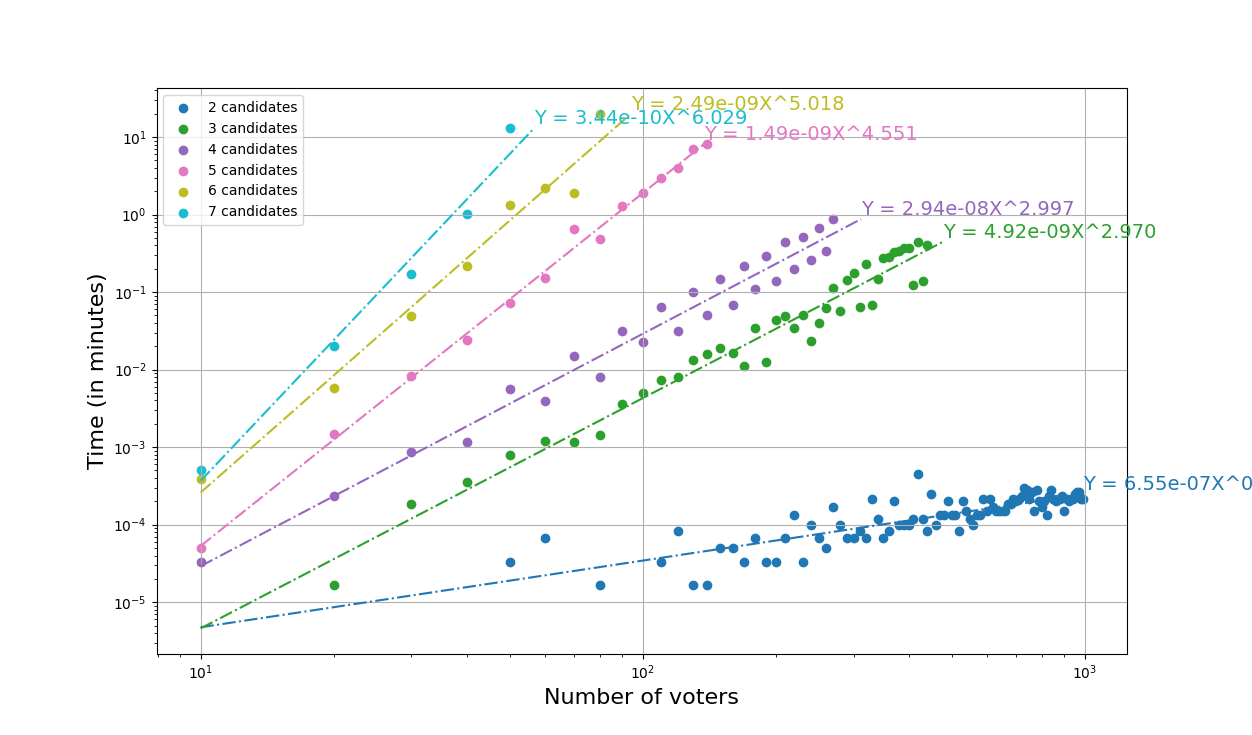
\includegraphics[width=.45\textwidth]{dlog-search.png}
%     \caption{Time required to solve DLP with respect to the number of candidates and number of voters (log-log scale).}
%     \label{fig:dlog-search}
% \end{figure}

\section{Deployments}
\label{sec:deployments}
The protocol can be deployed on any platform that supports a shared communication space (message board) where everyone can post and read messages. We consider three potential deployment scenarios:

\begin{enumerate}
    \item \textbf{Peer-to-peer Networks:} Our protocol is designed to be suitable for peer-to-peer networks, leveraging technologies such as Wesh Network\footnote{Wesh Network, asynchronous mesh network protocol powered by Berty Technologies' non-profit organisation, \url{https://wesh.network/}}, to provide a fully decentralized infrastructure.
    \item \textbf{Public Blockchains:}  The protocol can be implemented as a smart contract on a public blockchain using ERC-4337~\cite{ERC4337AccountAbstraction}, which enables centralized payment of transaction fees for all participants, thereby reducing the economic barrier for wider adoption.
    \item \textbf{Centralized Messengers}:  For ease of deployment, it is possible to use our protocol on centralized messenger platforms such as Telegram, Signal, or WhatsApp, where the chat room acts as a message board. Note that the centralized party might be able to exploit the censorship property of the system.
\end{enumerate}
Figure \ref{fig:stack-bc} visualizes three potential deployment scenarios.
\begin{figure}[h]
    \centering
    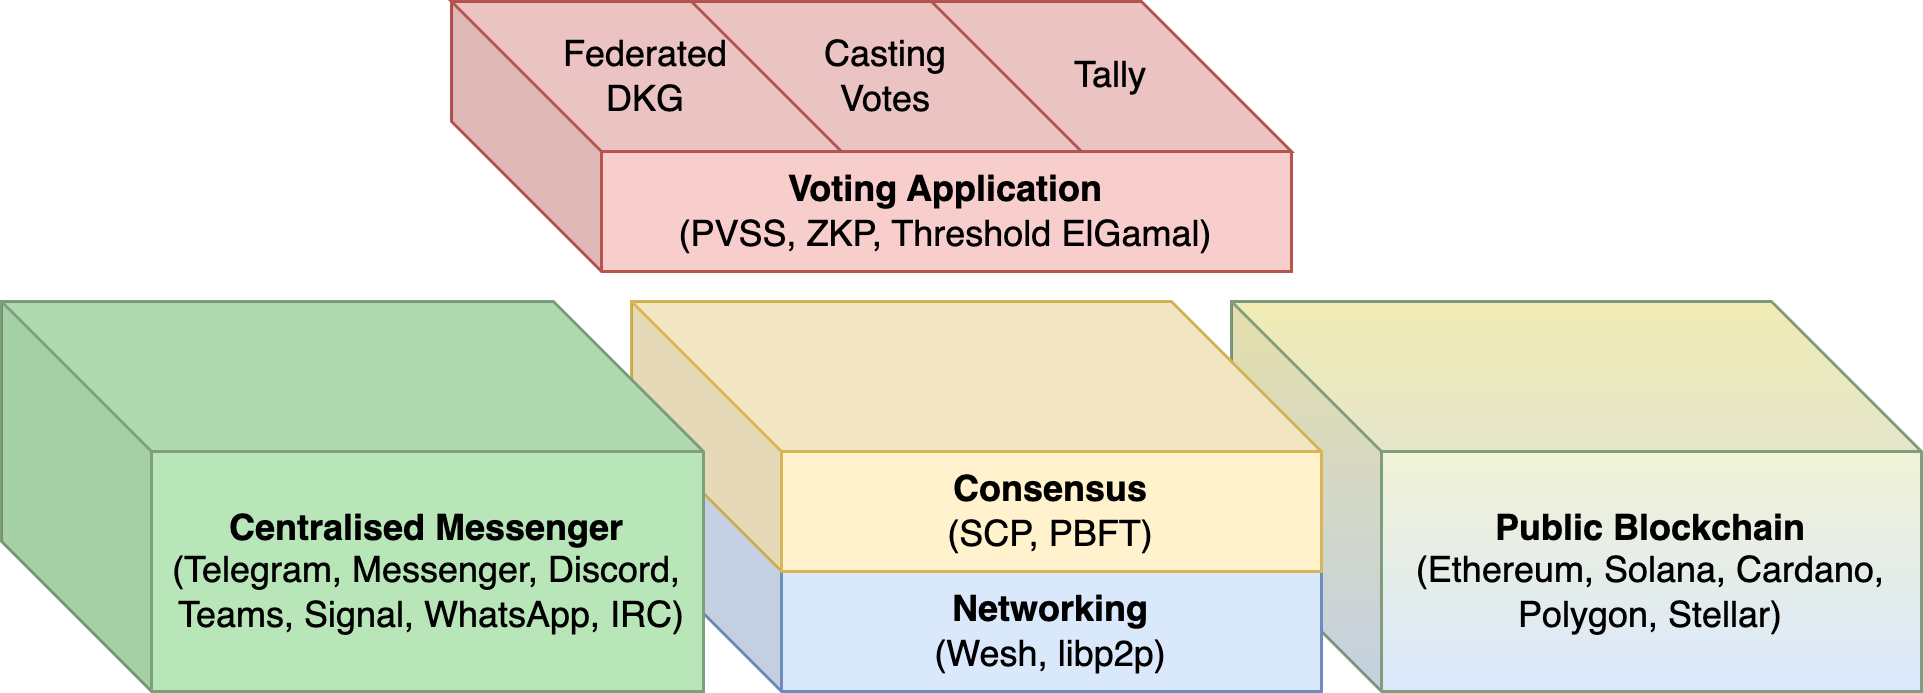
\includegraphics[width=0.5\textwidth]{stack-bc.png}
    \caption{Three possible deployments of the protocol: Centralised messenger, ad-hoc peer-to-peer network, and public blockchain.}
    \label{fig:stack-bc}
\end{figure}


% \section{Discussion and Conclusion}\label{sec:discussion-conclusion}

% \subsection{Discussion}

% Our FDKG scheme addresses a key challenge in decentralized settings: how to ensure reliable key reconstruction when not all parties are online or trustworthy. Traditional threshold DKG protocols assume a fixed number of participants with reliable availability, but in many real-world systems, network churn, node dropouts, and variability in trust relationships create practical barriers. By letting each participant define a personal guardian set, FDKG increases flexibility. When several nodes go offline, we can still reconstruct missing partial secrets if at least a threshold of guardians remain. This reduces bottlenecks caused by single points of failure or rigid, predefined trustee sets.

% We tested FDKG under different participation rates and guardian-set sizes, and we explored both Barabási–Albert and Random Graph trust structures. Results show that higher participation and retention rates (where more parties remain active through the key generation and reconstruction phases) naturally increase the probability of successful key reconstruction. Guardian sets that are too small risk losing shares if crucial members are offline. On the other hand, very large guardian sets can become impractical for users to manage (e.g., selecting dozens of guardians). These experiments suggest a balance: users who expect higher network churn may opt for slightly larger guardian sets for extra redundancy, while more stable groups can use smaller ones to reduce overhead. 

% From a performance standpoint, creating zero-knowledge proofs for partial key shares and verifying them adds computation and message overhead. Our measurements show that Groth16 can be used to keep proofs small and generation relatively fast, though proof times can reach a few seconds in more complex threshold settings. For large-scale elections with high candidate counts, we also note that the discrete-log search to decode final tallies might become a bottleneck. This could be mitigated using advanced discrete-log techniques or smaller candidate sets.

% A limitation of FDKG is that to protect privacy, all participants must ensure that no colluding group can satisfy both the threshold condition and Liveness requirements alone. In practical terms, users need to choose guardians who are unlikely to collude. When participants have heavily overlapping sets of guardians, a single adversary controlling those guardians might threaten privacy. Applying real-world reputation systems, social-graph data, or other trust signals can help users make robust guardian choices.

% Future research will focus on optimizing the computational cost of the discrete logarithm problem by employing more efficient algorithms, and exploring different consensus mechanisms for the message board to improve censorship resistance, while preserving the privacy and security of the FDKG.
% We believe that FDKG represents a valuable contribution to the field of decentralized voting, and that it is a foundational element for decentralized systems where trust should be shifted to the community rather than to a third party.

% \subsection{Conclusion}

% This paper introduced Federated Distributed Key Generation (FDKG), a generalization of traditional DKG that enables each party to select a personal guardian set for reconstructing its share of the secret key. Through simulations, we showed that FDKG retains the main security properties of threshold cryptography (liveness, safety, privacy) while offering flexibility and better resilience against node unavailability. We then illustrated how FDKG can serve as the foundation for a voter-to-voter internet voting scheme, improving decentralization by eliminating fixed authorities and single points of trust. 

% Our findings underscore that real-world conditions—such as varying participation rates, degrees of trust, and node churn—call for adaptive key generation strategies. FDKG aligns with these needs by allowing each participant to pick trusted guardians, and by tolerating absent participants in later phases. While some trade-offs remain, especially in choosing suitable guardian-set sizes and thresholds, FDKG represents a step toward more robust, user-centric cryptographic protocols. Its potential extends to broader applications in decentralized finance, secure multiparty computation, or any scenario where dynamic groups must share and protect cryptographic secrets. We provide an open-source reference implementation to facilitate further experimentation, adaptation, and real-world deployments.


\section{Limitations and Future Work}\label{sec:limitations-and-future}
Our implementation and simulations show that while FDKG substantially improves flexibility, it still inherits some cryptographic overhead. Although Groth16 proofs are efficient enough for mid-scale settings, large-scale or time-critical elections might demand faster proving systems or aggregated proofs. The offline tallying step in our voting example employs brute force to decode final votes; methods to reduce this overhead remain an open research challenge (e.g., more efficient multi-candidate encoding or advanced number-theoretic techniques). While our Barabási-Albert heuristics work well, a deeper exploration of context-aware selection strategies—possibly incorporating social or reputational metrics—would further strengthen the reliability and practical deployment of the protocol. Overall, these points open new avenues for research, particularly in optimizing the cryptographic building blocks and customizing guardian-set selection for varied application requirements.

Although the paper focuses on an i-voting application, the FDKG concept generalizes naturally to any setting where secret reconstruction and threshold cryptography are required but global membership is uncertain or shifts over time. Examples include collaborative data encryption in ad-hoc networks, decentralized credential management for distributed applications, and emergent governance structures (e.g., decentralized autonomous organizations).



\section{Discussion and conclusions}\label{sec:discussion-conclusion}

The FDKG protocol presented in this paper provides a novel, flexible approach to distributed key generation. Unlike standard DKG, which requires predefined sets of participants and threshold parameters, FDKG allows each participant to select its own guardian set of size $k$ without requiring prior knowledge of total network membership; this design ensures that liveness holds whenever the adversary cannot control both a participant and $k-t+1$ of its guardians.

FDKG generalizes traditional DKG by incorporating principles from Federated Byzantine Agreement (FBA), enabling dynamic trust delegation akin to the Stellar Consensus Protocol. Unlike dynamic DKG schemes requiring multiple rounds, FDKG achieves robustness in two phases, making it suitable for human-in-the-loop systems like voting. However, the reliance on zkSNARKs introduces trade-offs absent in non-verifiable DKG variants.

FDKG’s security assumes honest majority in guardian sets, which may not hold in sybil-prone environments. Additionally, the use of zkSNARKs necessitates trusted setups, a potential single point of failure. Future work could explore transparent proof systems (e.g., Bulletproofs) to mitigate this.

Simulations revealed that FDKG’s success rate depends heavily on participation (\(p\)) and retention (\(r\)) rates. For example, with \(n = 100\), \(p = 0.8\), and \(r = 0.9\), FDKG achieved a $100\%$ success rate for all thresholds $t$ lower than $0.7 k$. In contrast, lower retention (\(r = 0.5\)) achieved a $100\%$ success rate, only for small thresholds $t \leq 0.4 k$ (Figure~\ref{fig:guardian_configs}). The Barabási-Albert (BA) selection policy topology outperformed random selection, achieving a higher mean success rate by $\approx 0.025$ due to its hub-based resilience (Figure~\ref{fig:network_model}), the advantage however diminishes at larger networks i.e., $n>1000$.

While FDKG reduces reliance on global thresholds, it introduces communication overhead proportional to guardian set size. For \(n = 100\) participants, each with \(k = 40\) guardians, the Distribution Phase incurred 332.7 kB of data per participant. zkSNARKs, while essential for verifiability, added computational costs: proving times ranged from 3.36 seconds (\(k = 10\)) to 14.79 seconds (\(k = 100\)) (Table~\ref{table:proving-time}). These results underscore the need for parameter tuning based on deployment constraints—smaller \((k,t)\) for latency-sensitive applications, larger \((k,t)\) for adversarial environments.  


While smaller guardian sets reduce communication and computation costs, they also make each share holder’s availability more critical. Our security theorems show that an adversary controlling a participant and its $k - t$ nodes in any guardian set can endanger the liveness of the protocol. Hence, choosing too small a guardian set could inadvertently lower security if an attacker manages to compromise a higher fraction of those guardians. Balancing guardian set size against security requirements and node availability is therefore a key design parameter.

We envision FDKG as a versatile primitive for any multi-party setting that demands robust key distribution but faces incomplete or dynamic participation. Moving forward, optimizing zkSNARK proofs, refining the discrete log decoding in multi-candidate elections, and researching new guardian-set selection strategies can further extend the protocol’s usability. By embracing the decentralized and adaptive ethos at the core of FDKG, future systems can be built to scale securely across complex, real-world networks—ranging from small committee-style collaborations to massive global communities.

\section*{Reproducible Research}
We ensure reproducibility by providing all code, data, and scripts to regenerate results in Sections~\ref{sec:liveness_simulations} and \ref{sec:performance_evaluation}. These are hosted at \url{https://github.com/stanbar/PeerVote}, with a live simulator at \url{https://fdkg.stan.bar}. Instructions detail how to replicate simulation success rates (Figures~\ref{fig:guardian_configs}, \ref{fig:parameters_significance_participation}) and performance metrics (Table~\ref{table:proving-time}).

\section*{Acknowledgment}
We thank Lev Soukhanov for his early contributions to the FDKG concept and mechanics, and Oskar Goldhahn and Thomas Haines for their insightful reviews, enhancing the paper’s structure and cryptographic rigor.

\printbibliography
\section{Appendix}


\subsection{zkSNARK Constructions}\label{app:proofs}

In our protocol, we employ the general principles of zk-SNARK to construct specific proofs for each phase of the voting process. Each proof is defined by a circuit $C$ that verifies constraints, a public instance (statement) $\vec{s}$, and a private input (witness) $\vec{w}$.

\subsubsection{\ProofFDKG{i}}\label{app:proof-fdkg}

\begin{itemize}
    \item \textbf{Circuit} ($C$): Defined as \ProofFDKGInformal{}. The specifics of this circuit are detailed in Algorithm~\ref{alg:circuit_fdkg}.
    \item \textbf{Public Instance} ($\vec{s}$): Includes the partial encryption key $\PartialPublicKey{i}$, the guardian set $\GuardianSetOf{i} = \{\Party{1},\dots,\Party{|\GuardianSetOf{}|}\}$, and the set of encrypted partial decryption key shares $\{\EncryptedSharePartialSecretKey{}{1},\dots, \EncryptedSharePartialSecretKey{}{|\GuardianSetOf{}|}\}$.
    \item \textbf{Private Input} ($\vec{w}$): Includes the coefficients of the polynomial $\{a_0, \dots, a_{t-1}\}$ and random values $\{r1_1,\dots,r1_{|\GuardianSetOf{}|}\}$, $\{r2_1,\dots,r2_{|\GuardianSetOf{}|}\}$.
\end{itemize}

\subsubsection{\ProofPS{i}}\label{app:proof-ps}

\begin{itemize}
    \item \textbf{Circuit} ($C$): Defined as ``Given $\PartialPublicKey{i}$, I know a partial secret key $\PartialSecretKey{i}$ s.t. $\PartialPublicKey{i} = \PartialSecretKey{i} G$''. The specifics of this circuit are detailed in Algorithm~\ref{alg:circuit_proof_ps}.
    \item \textbf{Public Instance} ($\vec{s}$): Includes the partial encryption key $\PartialPublicKey{i}$.
    \item \textbf{Private Input} ($\vec{w}$): Includes the partial decryption key $\PartialSecretKey{i}$.
\end{itemize}

\subsubsection{\ProofSPS{i}{j}}\label{app:proof-sps}

\begin{itemize}
    \item \textbf{Circuit} ($C$): Defined as ``Given $\SharePartialSecretKey{j}{i}$, $\EncryptedSharePartialSecretKey{j}{i}$, $\Delta$ I know a partial secret key $\PartialSecretKey{i}$ s.t. $\PartialPublicKey{i} = \PartialSecretKey{i} G$ and  $\SharePartialSecretKey{j}{i} = \DecryptionUsingOf{\PartySecretKey{i}}{\EncryptedSharePartialSecretKey{j}{i}}$''. The specifics of this circuit are detailed in Algorithm~\ref{alg:circuit_proof_sps}.
    
    \item \textbf{Public Instance} ($\vec{s}$): Includes the share of partial secret key $\SharePartialSecretKey{j}{i}$, the encrypted partial decryption key share $\EncryptedSharePartialSecretKey{j}{i}$, and the difference $\Delta$.
    
    \item \textbf{Private Input} ($\vec{w}$): Includes the secret key of party $\PartySecretKey{i}$.
\end{itemize}


\begin{algorithm}
\caption{Circuit FDKG(k = guardian set size, t = threshold)}
\label{alg:circuit_fdkg}

\KwIn{Statement $\vec{s}: (\PartialPublicKey{i}, \GuardianSetOf{} = \{\Party{1},\dots,\Party{|\GuardianSetOf{}|}\}, \{\EncryptedSharePartialSecretKey{}{1},\dots, \EncryptedSharePartialSecretKey{}{|\GuardianSetOf{}|} \})$}

\KwIn{Witness $\vec{w}: (\{a_0, \dots, a_{t-1}\}, \{r1_1,\dots,r1_{|\GuardianSetOf{}|}\}, \{r2_1,\dots,r2_{|\GuardianSetOf{}|}\})$}

\SetKwFunction{Num2Bits}{Num2Bits}
\SetKwFunction{EscalarMulFix}{EscalarMulFix}
\SetKwFunction{EscalarMulAny}{EscalarMulAny}
\SetKwFunction{BabyAdd}{BabyAdd}
\SetKw{KwTo}{to}
\SetKw{KwIn}{in}
\SetKw{KwDownTo}{down to}
\SetKw{KwAssert}{assert}
\SetKw{BaseOrder}{q}
\SetKwData{Threshold}{t}
\SetKwData{Eval}{eval}
\SetKwData{GuardianSetSize}{$|\GuardianSetOf{}|$}


\SetKw{Assert}{assert}

\BlankLine

\Assert \PartialPublicKey{i} = \EscalarMulFix{\PartySecretKey{i}, \G}\;

\For{i \KwIn \GuardianSetSize}{
    $\Eval[i][0] \leftarrow a_0$\;
    \For{j \KwIn \Threshold}{
        e $\leftarrow (i+1)^j\ \%\ \BaseOrder$\;
        d $\leftarrow (a_j \cdot  e)\ \%\ \BaseOrder$\;
        $\Eval[i][j] \leftarrow (\Eval[i][j-1] + d)\ \%\ \BaseOrder$\;
    }
    
    $R \leftarrow \EscalarMulAny(r1_i, \Party{i})$\; % party in guardiansPubKeys[i]
    
    $F \leftarrow \EscalarMulFix(r2_i, \G)$\;
    
    $J \leftarrow \BabyAdd(R, F)$\;
    $\Delta \leftarrow F_x - \Eval[i][\Threshold]$\;

    \Assert $\EncryptedSharePartialSecretKey{}{i}.C1 = \EscalarMulFix{r1[i], \G}$\;
    \Assert $\EncryptedSharePartialSecretKey{}{i}.C2 = J$\;
    \Assert $\EncryptedSharePartialSecretKey{}{i}.\Delta = \Delta$\;
}
\end{algorithm}

\begin{algorithm}[h!]
\caption{Circuit PartialSecret}
\label{alg:circuit_proof_ps}

\KwIn{Statement $\vec{s}: (\PartialPublicKey{i})$}
\KwIn{Witness $\vec{w}: (\PartialSecretKey{i})$}
\SetKwFunction{Num2Bits}{Num2Bits}
\SetKwFunction{EscalarMulFix}{EscalarMulFix}
\SetKwFunction{EscalarMulAny}{EscalarMulAny}
\SetKwFunction{BabyAdd}{BabyAdd}
\SetKw{KwTo}{in}
\SetKw{KwDownTo}{down to}
\SetKw{Assert}{assert}

\BlankLine

\Assert $\PartialPublicKey{i} = \EscalarMulFix{\PartialSecretKey{i}, \G}$\;
\end{algorithm}


\begin{algorithm}[h!]
\caption{Circuit SharePartialSecret}
\label{alg:circuit_proof_sps}

\KwIn{Statement $\vec{s}: (\SharePartialSecretKey{j}{i}, \EncryptedSharePartialSecretKey{j}{i}, \Delta)$}
\KwIn{Witness $\vec{w}: (\PartySecretKey{i})$}
\SetKwFunction{Num2Bits}{Num2Bits}
\SetKwFunction{EscalarMulFix}{EscalarMulFix}
\SetKwFunction{EscalarMulAny}{EscalarMulAny}
\SetKwFunction{BabyAdd}{BabyAdd}
\SetKwFunction{Assert}{Assert}
\SetKw{KwTo}{in}
\SetKw{KwDownTo}{down to}
\SetKw{Assert}{assert}

\BlankLine

$X \leftarrow \EscalarMulAny(\PartySecretKey{i}, \EncryptedSharePartialSecretKey{j}{i}[1])$\; % s_i C_1

$(M_x, M_y) \leftarrow \BabyAdd(\EncryptedSharePartialSecretKey{j}{i}[2], - X)$\; % M = C_2 - s_i C_1

\Assert $\SharePartialSecretKey{j}{i} = M_x - \Delta$\;

\end{algorithm}

\subsubsection{\ProofBALLOT{i}}\label{app:proof-ballot}

\begin{itemize}
    \item \textbf{Circuit} ($C$): Defined as \ProofBALLOTInformal{}. Algorithm~\ref{alg:circuit_proof_ballot} elaborates on this circuit.
    \item \textbf{Public Instance} ($\vec{s}$): Includes the encryption key $\PublicKey{}$ and the encrypted ballot $\Ballot{i} = (C1, C2)$.
    \item \textbf{Private Input} ($\vec{w}$): Includes the vote $\Vote{i}$ and the random blinding factor $r_i$.
\end{itemize}

\subsubsection{\ProofPD{i}}\label{app:proof-pd}

\begin{itemize}
    \item \textbf{Circuit} ($C$): Specified as \ProofPDInformal{}. Details of this circuit can be found in Algorithm~\ref{alg:circuit_proof_pd}.
    \item \textbf{Public Instance} ($\vec{s}$): Includes the sum of first ballot components $\TotalA{}$, the partial decryption from party $\PartialDecryptionFrom{i}$, and the partial encryption key $\PartialPublicKey{i}$.
    \item \textbf{Private Input} ($\vec{w}$): Includes the partial decryption key $\PartialSecretKey{i}$.
\end{itemize}

\subsubsection{\ProofPDS{i}{j}}\label{app:proof-pds}

\begin{itemize}
    \item \textbf{Circuit} ($C$): Outlined as \ProofPDSInformal{}. For more information, refer to Algorithm~\ref{alg:circuit_proof_pds}.
    \item \textbf{Public Instance} ($\vec{s}$): Includes the sum of first ballot components $\TotalA{}$, the share of partial decryption $\SharePartialDecryptionFromTo{j}{i}$, the encrypted partial decryption key share $\EncryptedSharePartialSecretKey{j}{i}$, and the difference $\Delta$.
    \item \textbf{Private Input} ($\vec{w}$): Includes the secret key of party $\PartySecretKey{i}$.
\end{itemize}



\begin{algorithm}[h!]
\caption{Circuit EncryptedBallot(m = the smallest integer s.t. $2^m > |\mathbb{P}|$ )}
\label{alg:circuit_proof_ballot}

\KwIn{Statement $\vec{s}: (\PublicKey{}, \Ballot{i} = (C1, C2) )$}
\KwOut{Witness $\vec{w}: (\Vote{i}, r)$}

\SetKwFunction{Num2Bits}{Num2Bits}
\SetKwFunction{EscalarMulFix}{EscalarMulFix}
\SetKwFunction{EscalarMulAny}{EscalarMulAny}
\SetKwFunction{BabyAdd}{BabyAdd}
\SetKw{KwTo}{in}
\SetKw{KwDownTo}{down to}
\SetKw{Assert}{assert}

% \KwAssert{$options > 1$}\;
% \KwAssert{$1 \leq \Vote{i} \leq options$}\;
% \KwAssert{$m > 2^{voters}$}\;

\BlankLine

\Assert $C1 = \EscalarMulFix{r, \G}$\;

F $\leftarrow$ \EscalarMulAny{r, \PublicKey{}}\;

e $\leftarrow$ $2^{(\Vote{i} - 1) m}$\;

H $\leftarrow$ \EscalarMulFix{e, \G}\;

\Assert $C2 = \BabyAdd{F, H}$\;

\end{algorithm}


\begin{algorithm}[h!]
\caption{Circuit PartialDecryption}
\label{alg:circuit_proof_pd}

\KwIn{Statement $\vec{s}: (\TotalA{}, \PartialDecryptionFrom{i}, \PartialPublicKey{i})$}
\KwIn{Witness $\vec{w}: (\PartialSecretKey{i})$}
\SetKwFunction{Num2Bits}{Num2Bits}
\SetKwFunction{EscalarMulFix}{EscalarMulFix}
\SetKwFunction{EscalarMulAny}{EscalarMulAny}
\SetKwFunction{BabyAdd}{BabyAdd}
\SetKw{KwTo}{in}
\SetKw{KwDownTo}{down to}
\SetKw{Assert}{assert}

\BlankLine

\Assert $\PartialPublicKey{i} = \EscalarMulFix{\PartialSecretKey{i}, \G}$\;
\Assert $\PartialDecryptionFrom{i} = \EscalarMulAny{\PartialSecretKey{i}, \TotalA{}}$\;
\end{algorithm}


\begin{algorithm}[h!]
\caption{Circuit PartialDecryptionShare}
\label{alg:circuit_proof_pds}

\KwIn{Statement $\vec{s}: (\TotalA{}, \SharePartialDecryptionFromTo{j}{i}, \EncryptedSharePartialSecretKey{j}{i}, \Delta)$}
\KwIn{Witness $\vec{w}: (\PartySecretKey{i})$}
\SetKwFunction{Num2Bits}{Num2Bits}
\SetKwFunction{EscalarMulFix}{EscalarMulFix}
\SetKwFunction{EscalarMulAny}{EscalarMulAny}
\SetKwFunction{BabyAdd}{BabyAdd}
\SetKwFunction{Assert}{Assert}
\SetKw{KwTo}{in}
\SetKw{KwDownTo}{down to}
\SetKw{Assert}{assert}

\BlankLine

$X \leftarrow \EscalarMulAny(\PartySecretKey{i}, \EncryptedSharePartialSecretKey{j}{i}[1])$\; % s_i C_1

$(M_x, M_y) \leftarrow \BabyAdd(\EncryptedSharePartialSecretKey{j}{i}[2], - X)$\; % M = C_2 - s_i C_1

$\SharePartialSecretKey{j}{i} \leftarrow M_x - \Delta$\;

\Assert $\SharePartialDecryptionFromTo{j}{i} = \EscalarMulAny(\SharePartialSecretKey{j}{i}, \TotalA{})$
\end{algorithm}




\end{document}